\documentclass[UTF8]{ctexart}
\usepackage{xcolor}
\usepackage{listings}
\usepackage{booktabs}
\usepackage{float}
\usepackage{graphicx}
\usepackage{subfigure}
\usepackage{amsmath}
\allowdisplaybreaks
\title{“归纳主义者的错觉” \\ \hspace*{\fill} \\ 基于元胞自动机的新冠病毒传播研究}
\author{\\高成志\\ 张彬 \\李以煌}
\date{\today}
\begin{document}
\maketitle

\newpage
\begin{abstract}
    % 摘要
    \par 
    新型冠状病毒疫情对全国造成了严重影响,人民的生产生活受到极大损失。应用数学建模方法对病毒传播过程和政府防疫手段进行科学有效的定量分析与评估具有重要意义。
    \par 
    本文基于SEIR病毒传播模型对国内的病毒传播数据进行了定量分析,并对各省新冠传播的速度、控制措施的有效性作出了综合评估。通过数据分析,对比了中国新冠病毒传播与美国新冠病毒传播的区别。针对美国疫情的发展特点建立了元胞自动机模型模拟疫情后续的发展趋势,并依据模型生成的数据预测了美国6月份的病毒感染人数。
    \par 
    通过对比模型数据与实际数据我们发现,SERI模型对中国新冠病毒的传播趋势模拟较好。病毒扩散在短时间内得到控制充分反映出了中国防疫方案的先进性和有效性,为全球其他国家掌控干预节奏、制定防控策略提供了有益参考。而元胞自动机模型则难以预测变化多端的美国疫情发展,我们的预测结果过于乐观,与现实严重不符。针对这一现象我们进行了深刻的反思。
    \\ \hspace*{\fill} \\  
    \textbf{关键词}:新型冠状病毒 ;SEIR ;元胞自动机 ;动态调优 ;数学建模
\end{abstract}
\newpage

\tableofcontents

\newpage
% 正文
\section{问题背景与重述}
\subsection{问题背景} % (fold)
\label{sub:问题背景}
2020年初,一场由新型冠状病毒引发的疫情在武汉迅速传播,并逐渐蔓延到全国,
人民的生产生活受到了极其严重的负面影响。
党中央领导高度重视,立即采取了强有力的防治措施,
在各级人民政府的协同行动和广大人民群众的积极配合之下,
国内的疫情很快得到了初步的控制。
\par
与此同时,新型冠病毒继续向海外扩散。
疫情在几个主要的西方国家(尤其是美国)并没有得到很好的控制。
特别是进入六月以来,随着以美国为首的西方国家不断爆发大规模的反种族主义抗议游行,
使得原本快要被遏制的疫情又有了反扑的可能。
\par
截至北京时间6月11日7时42分,全球新冠状病毒确诊病例达7,347,323例,死亡病例为415,174例。美国确诊病例达1,997,636例,死亡病例为112,769例。这些数字还在不断的增长中。

% subsection1.1	问题背景 (end)

\subsection{需解决的问题:}
\begin{enumerate}
    \item 分析国内的病毒传播数据(统计描述)。 
    \item 综合评估各省新冠传播的速度、控制措施的有效性。 
    \item 通过数据分析对比中国新冠传播与美国新冠传播的区别。
    \item 预测美国新冠感染人数在六月份的数据。 
\end{enumerate}
\section{问题分析}
对于第一个问题,我们将汇总全国疫情新增、死亡、治愈人数的统计数据,使用 SEIR 模型对新冠疫情进行模拟,调整参数进行拟合,得出针对国内的病毒传播的统计描述。
\par 对于第二个问题,我们将收集各省疫情发展情况的统计数据,运用批处理工具,生成各省疫情发展曲线进行对比,给出概括性的传播特征结论。对疫情控制措施的有效性进行定量分析。
\par 对于第三个问题,我们将结合美国疫情发展的统计数据,对比中国新冠疫情的传播特征,找出两者的异同点,并尝试进行分析。
\par 对于第四个问题,我们将结合六月之前的疫情增长情况,运用建立元胞自动机模型进行预测。再针对六月初的疫情数据,对模型的参数进行动态调优拟合,得出美国新冠感染人数在六月份的预测数据,最后与实际情况进行对比。


\section{模型假设}
\subsection{假设条件}
\begin{enumerate}
    \item   假设收集的数据能客观公正地表现疫情的实际情况。
    \item 	感染系数 $\beta$ 在封城后保持不变。
    \item 	患者的恢复系数 $\gamma$ 保持不变。
    \item 	潜伏者的发病概率 $\alpha$ 保持不变。
\end{enumerate}

\subsection{符号说明}

\begin{table}[htbp]
    \centering
    \setlength{\tabcolsep}{1.8cm}{
    \begin{tabular}{c|c}
    \toprule
    符号         & 解释                \\
    \midrule
    S           & 易感者 (Susceptible) \\
    E           & 暴露者 (Exposed)     \\
    I           & 感病者 (Infectious)  \\
    R           & 康复者 (Recovered)   \\
    r           & 感染患者(I)每天接触的易感者数目 \\
    $\beta$     & 传染系数              \\
    $\alpha$    & 潜伏者的发病概率          \\
    t           & 时间间隔的单位,默认为天      \\
    % N           & 初始全体人数            \\
    % L           & 元胞空间              \\
    % d           & 元胞自动机内元胞空间的维数     \\
    % $N_1$       & 某个邻域内所有元胞的集合     \\
    % f           & 局部映射或局部规则        \\ 
    \bottomrule
    \end{tabular}}
    \end{table}



\subsection{图表说明}

\begin{table}[]
    \centering
    \setlength{\tabcolsep}{1.8cm}{
    \begin{tabular}{c|c}
    \toprule
    符号                    & 解释                                \\
    \midrule
    total                 & 累计确诊人数                            \\
    Increased             & 新增人数                              \\
    InfectedNow           & 现有确诊人数                            \\
    death                 & 累计死亡人数                            \\
    cure                  & 累计治愈人数                            \\
    HMT                   & 港澳台累计确诊人数                         \\
    abroad                & 境外累计确诊人数                          \\
    positive              & 美国累计确诊                            \\
    negative              & 美国检测后成阴性                          \\
    \bottomrule
    \end{tabular}}
    \end{table}

\subsection{数据来源\&采集}
国内数据clone自GitHub 相关数据收集仓库\cite{bib1},
使用Perl 运用正则表达式进行数据剔除,修正了不正确的xlsx 数据格式。
美国疫情数据来源于教师提供的dailyAmerican.xlsx表格和美国疾控中心(CDC)官网\cite{usaCdc}的数据。
\\
\par 经过滤后国内数据的表头为:
\\
 时间 | 确诊人数总和 | 新增人数 | 现有确诊人数 |
死亡人数 | 治愈人数	 | 港澳台共计 | 累计境外输入
\\
\par 各省数据表格的表头为:
\\
Province | State | Confirmed | Death | Recovered
\\
\par 美国疫情数据的表头为:
\\
date | states | positive | negative | pending | hospitalizedCurrently | hospitalizedCumulative | inIcuCurrently | inIcuCumulative | onVentilatorCurrently | onVentilatorCumulative | recovered | dateChecked | death | hospitalized | lastModified | total | totalTestResults | posNeg | deathIncrease | hospitalizedIncrease | negativeIncrease | positiveIncrease | totalTestResultsIncrease 
\\\hspace*{\fill}\\
\subsection{国内病毒传播数据的统计分析}

\subsubsection{数据处理}
首先我们依据处理后的表格meta.xlsx绘制出了中国新冠疫情发展的85天趋势图
(数据统计开始于2020年1月10号,截止于2020年4月3号),
代码见附录domestic.m 文件。

\par
我们可以很清楚的看到,在第34天,数据有了明显的异常(图2)波动:
\begin{figure}[htbp]
\centering
\begin{minipage}[t]{0.48\textwidth}
\centering
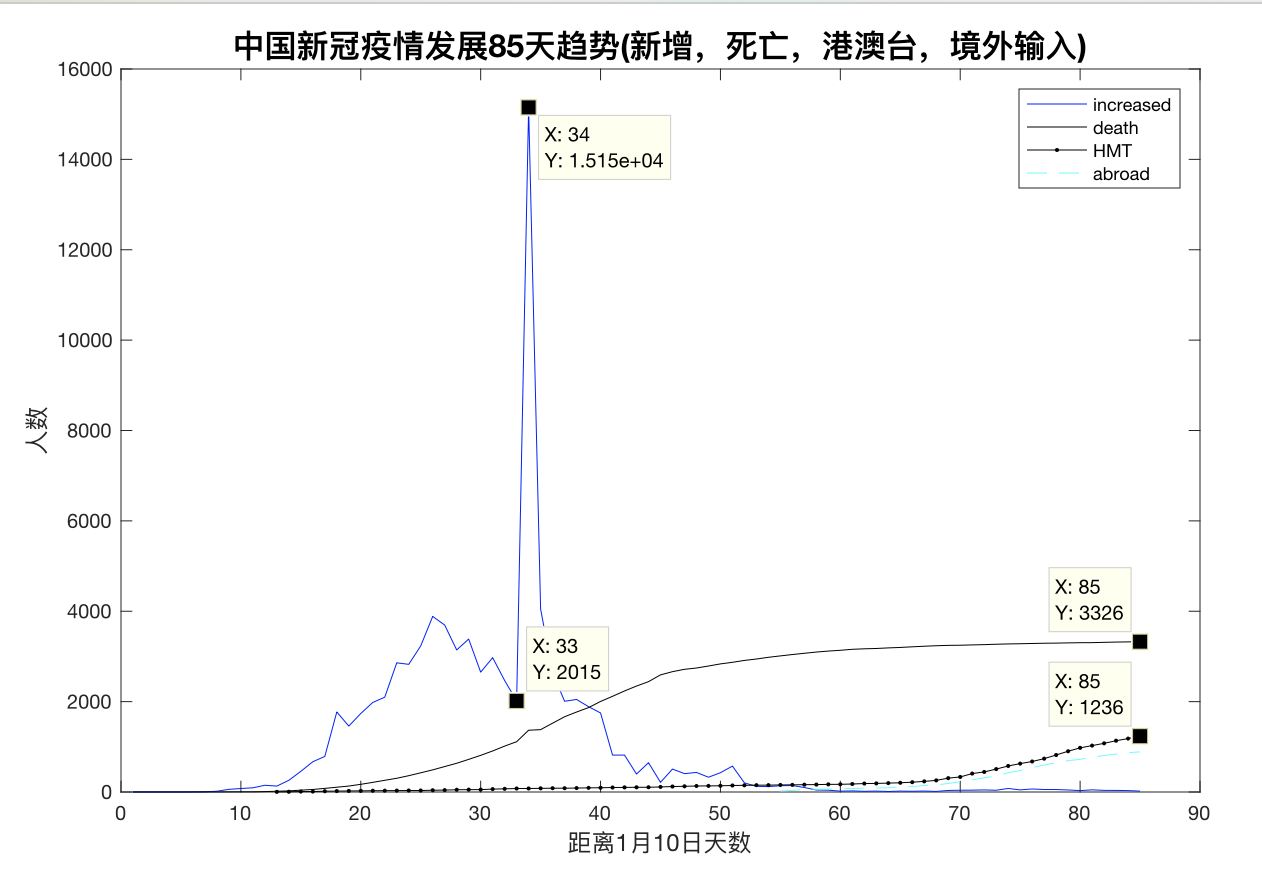
\includegraphics[width=6cm]{2.png}
\caption{中国新冠疫情发展趋势}
\end{minipage}
\begin{minipage}[t]{0.48\textwidth}
\centering
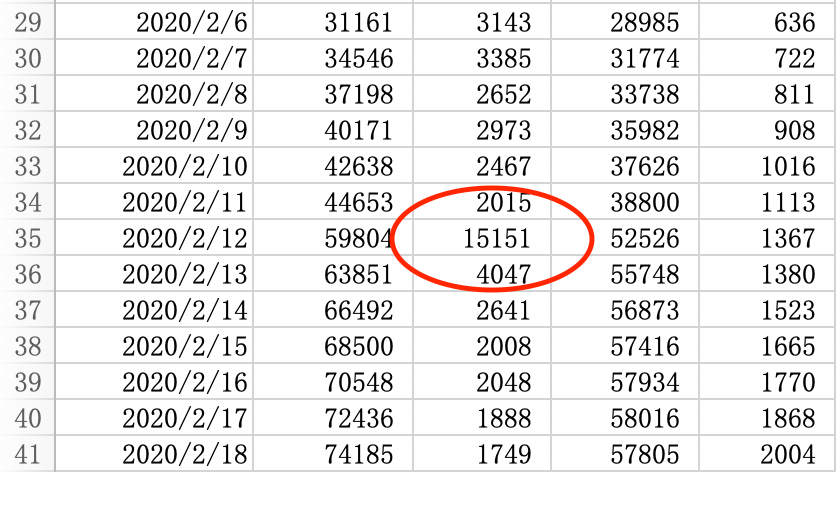
\includegraphics[width=6cm]{excel.png}
\caption{数据变更说明图}
\end{minipage}
\end{figure}
\par 


这是由于当天疫情统计部门临时更换统计策略造成的。
\\
\par 
为了更好地减少由于政策变更对统计数据造成的测量影响,
我们将第34、35 两天的数据做了平滑处理,
处理后的数据依据数字数量级分为A、B两图重绘如下:

\begin{figure}[htbp][H]
\centering
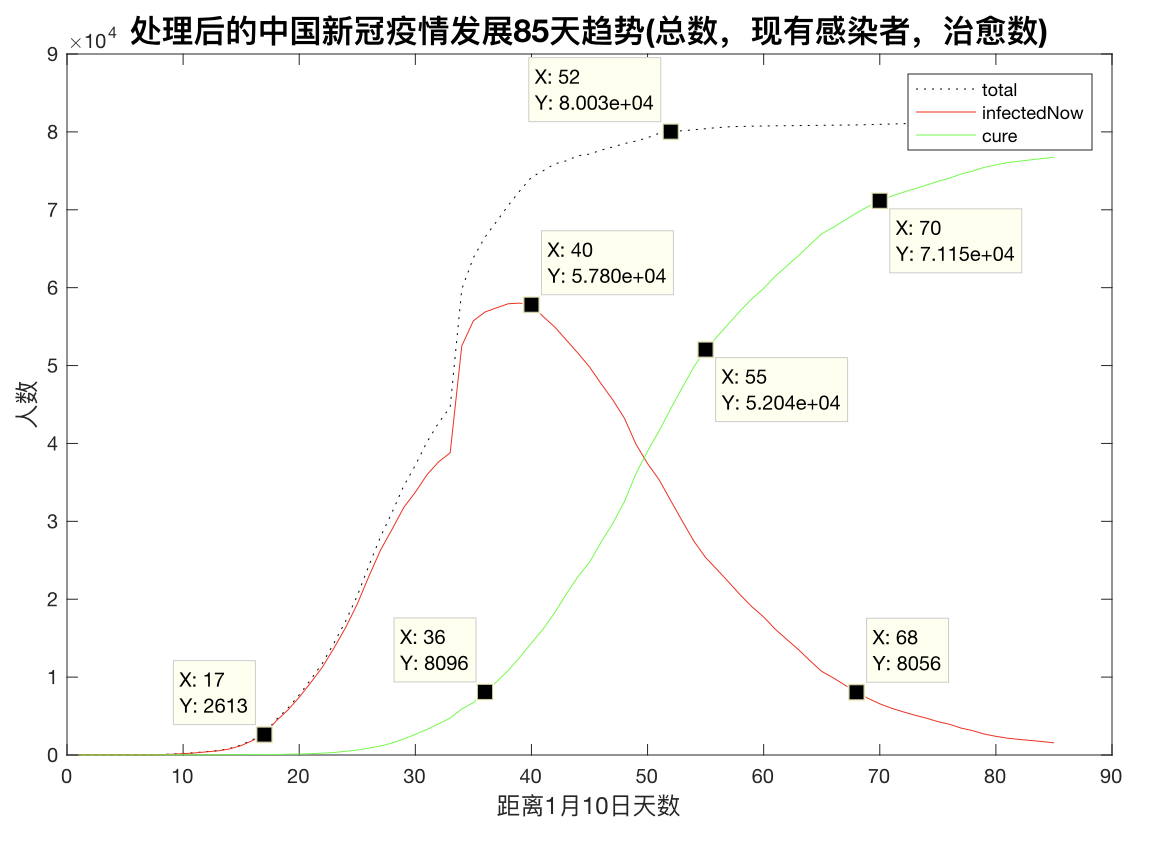
\includegraphics[width=8cm]{3.png} 
\caption{处理后的中国新冠疫情发展趋势A}
\end{figure}
\par

从A图可以看出,累计确诊人数在统计数据开始后的第52 天(3月1号)到达
增长顶点(80,026人),随后进入平台期,标志着国内疫情基本得到控制。
\par 
而现有确诊人数自统计第17天(1月26日)以来迅速增长,
到第40天(2月18日)到达增长顶点(57,805人),随后快速下降,
到第68天开始下降速度开始放缓。
康复人数的大幅增加的时间段正位于现有确诊人数快速下降的阶段。
\begin{figure}[htbp][H]
    \centering
    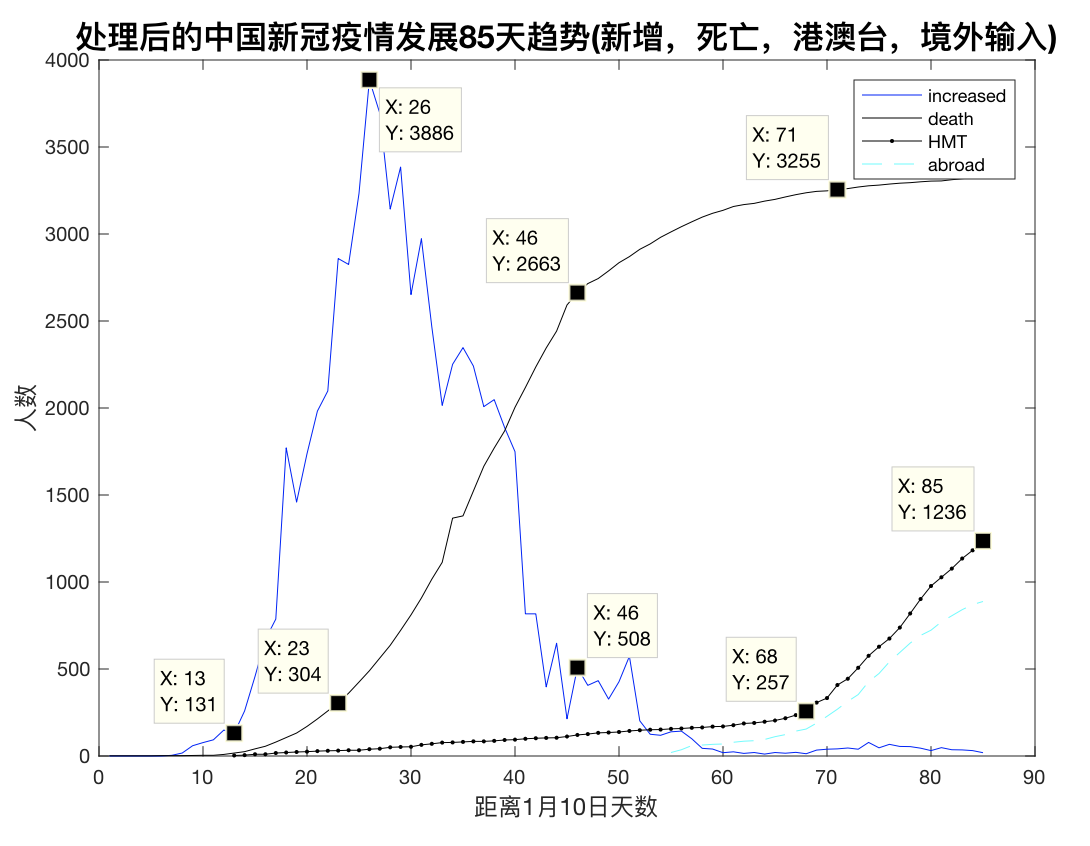
\includegraphics[width=8cm]{4.png} 
    \caption{处理后的中国新冠疫情发展趋势B}
\end{figure}
\par
从B 图中我们可以看出,新增人数从开始统计(1月1日)时的大幅上升到从第26天
(2月4日)开始大幅下降,整个转变过程非常剧烈,并不符合传统病毒传播模型的一般曲线。
\par 
结合武汉的封城日期(1月23号)我们推测:
这是由于疫情初期的病毒传播没有受到地方防疫部门的足够重视,
又恰好赶上春运的大规模人员流动,给病毒急剧传播营造了有利条件,
因此了非常陡峭的增长曲线。
而之后的城市封锁又以一种极端的方式瞬间锁死了人员流量,
从源头切断了病毒传播,造成了如图所示的急剧下降的新增人数曲线。
\par 
可以发现,封锁交通在疫情初期的效果也并不是立竿见影的,
而是有一个过程,大概在七天左右。
\par 
比较有意思的是到第68天(3月17日),
港澳台确诊和境外输入的病例明显开始上涨,
这标志着新冠病毒开始向外国扩散。
关于这部分的内容分析我们将把它留在国外疫情部分。
\par 
接下来我们将对疫情传播进行数学建模。

\subsubsection{SEIR传染病模型的描述}
SETR 传染病模型是一种常见的病毒传播模型,它将人群分为以下四个主要部分:
\begin{enumerate}
    \item S类人群,指的是病毒易感人群(Susceptible),尚未感染病毒,但缺乏病毒免疫能力,与病毒感染者接触后容易感染病毒。
    \item E 类人群,指的是接触过感染者 I ,暂无能力传染其他人的类,暴露(Exposed)在公共环境中,适用于潜伏期较长的传染疾病。
    \item I 类人群,感染者(Infections),感染过病毒,并有较大概率传播给S 类人群,将其转化成 I或 E 类人群。
    \item R 类人群,康复或移除(Removed or Recovered),通常病人康复或死亡后均不具有明显感染能力,故将该类人群移除出统计范围。
\end{enumerate}

\par 四者转化关系的参数为:
\begin{enumerate}
    \item   r为感染患者I 每天接触的易感人群的数目,初始值设置为30。
    \item 	$\beta$ 为传染系数,暴露人群被感染的可能性,初始值设置为0.03。
    \item 	$\gamma$ 为恢复系数,通常设置为康复时间的倒数,这里设置成0.1。 
    \item 	$\alpha$ 潜伏者的发病概率,通常设置成患者潜伏期的倒数,这里设置成 0.1。
    \item   t为时间度量的离散间隔,设置为85 个单位(天)。
    \item   N为初始的全体人数。
\end{enumerate}

\begin{figure}[htbp][H]
\centering
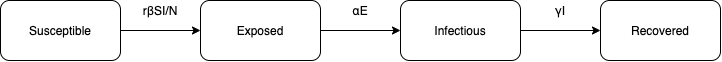
\includegraphics[width=8cm]{liu.png} 
\caption{转换流程图}
\end{figure}
\par

转化的方式是:
\\\hspace*{\fill}\\
$$
\begin{aligned}
\frac{d S}{d t}&=\frac{-r \beta I S}{N} \\
\frac{d E}{d t}&=\frac{r \beta I S}{N}-\alpha \mathrm{E} \\
\frac{d I}{d t}&=\alpha \mathrm{E}-\gamma \mathrm{I} \\
\frac{d R}{d t}&=\gamma I
\end{aligned}
$$
\\\hspace*{\fill}\\
当 dt=1 时,上式的离散形式表现为:
\\\hspace*{\fill}\\
$$
\begin{aligned}
S_{t+1}-S_{t}&=\frac{-\gamma \beta I_{t} S_{t}}{N} \\
E_{t+1}-E_{t}&=\frac{\gamma \beta I_{t} S_{t}}{N-\alpha E_{t}} \\
I_{t+1}-I_{t}&=\alpha E_{t}-\gamma I_{t} \\
R_{t+1}-R_{t}&=\gamma I_{t}
\end{aligned}
$$

\subsubsection{模型实现}
据此我们编写了matlab 程序(代码见附录simulation.m 部分)
来展示SEIR 模型模拟下的病毒传播趋势(图6)。

\begin{figure}[htbp][H]
\centering
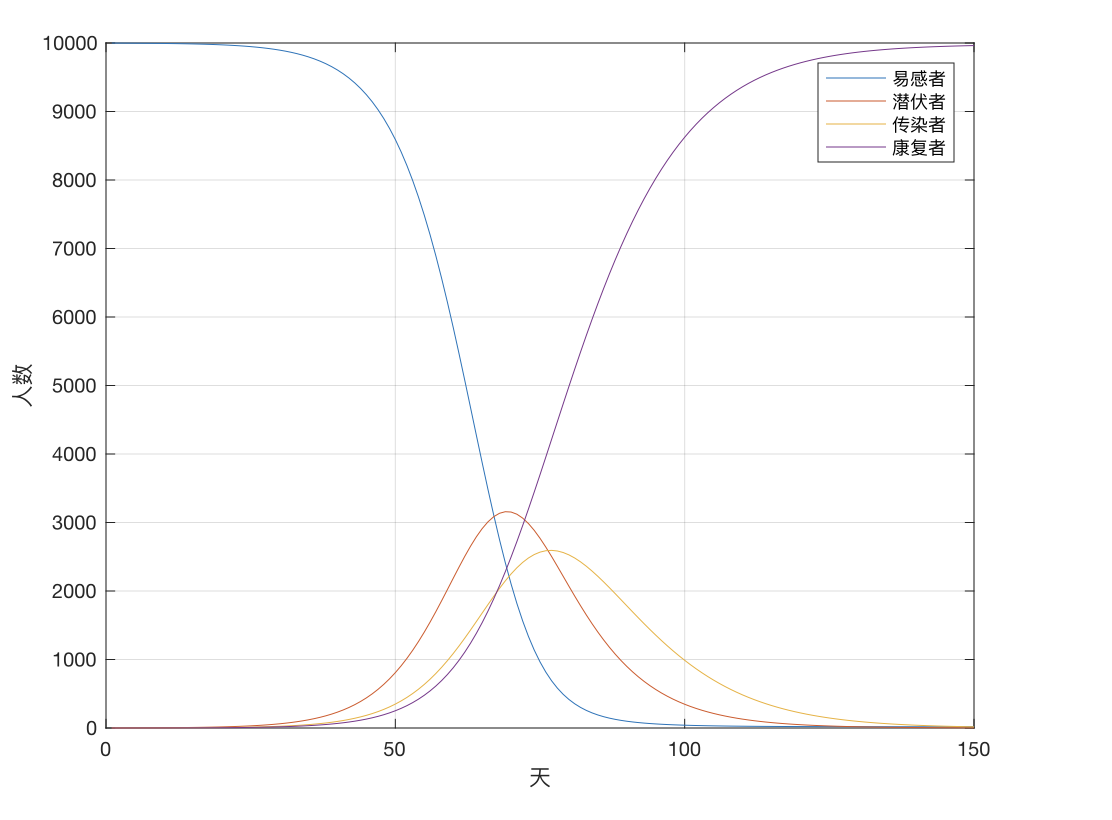
\includegraphics[width=8cm]{5.png} 
\caption{SEIR 模型的病毒传播趋势}
\end{figure}
\par
这是一个非常漂亮的理论模拟曲线,但是它有一些问题:
\\
\begin{enumerate}
    \item 全国疫情的重灾区是武汉地区,而武汉是一座有着1400万 人口\cite{bib2} 的大都市,本模型的初始人口数据明显偏小了,为后面的曲线拟合带来了麻烦。
    \item 模型的增长曲线非常光滑,这是由于没有考虑封城给病毒传播带来的影响造成的,这不符合实际新冠病毒的发展趋势。
    \item 由于人口基数过小,最终被感染的人数的比例明显偏高了,人口调整后之后总人口在数值上变化不明显,对后期比较是一个干扰项。
\end{enumerate}
\par 
针对以上的种种问题,我们修改了程序(代码见附录simulation2.m 部分)
增加了初始人数,设置了封城的触发条件,调节了相关参数,重新绘制了模拟曲线图。(图7)\\

\begin{figure}[htbp][H]
\centering
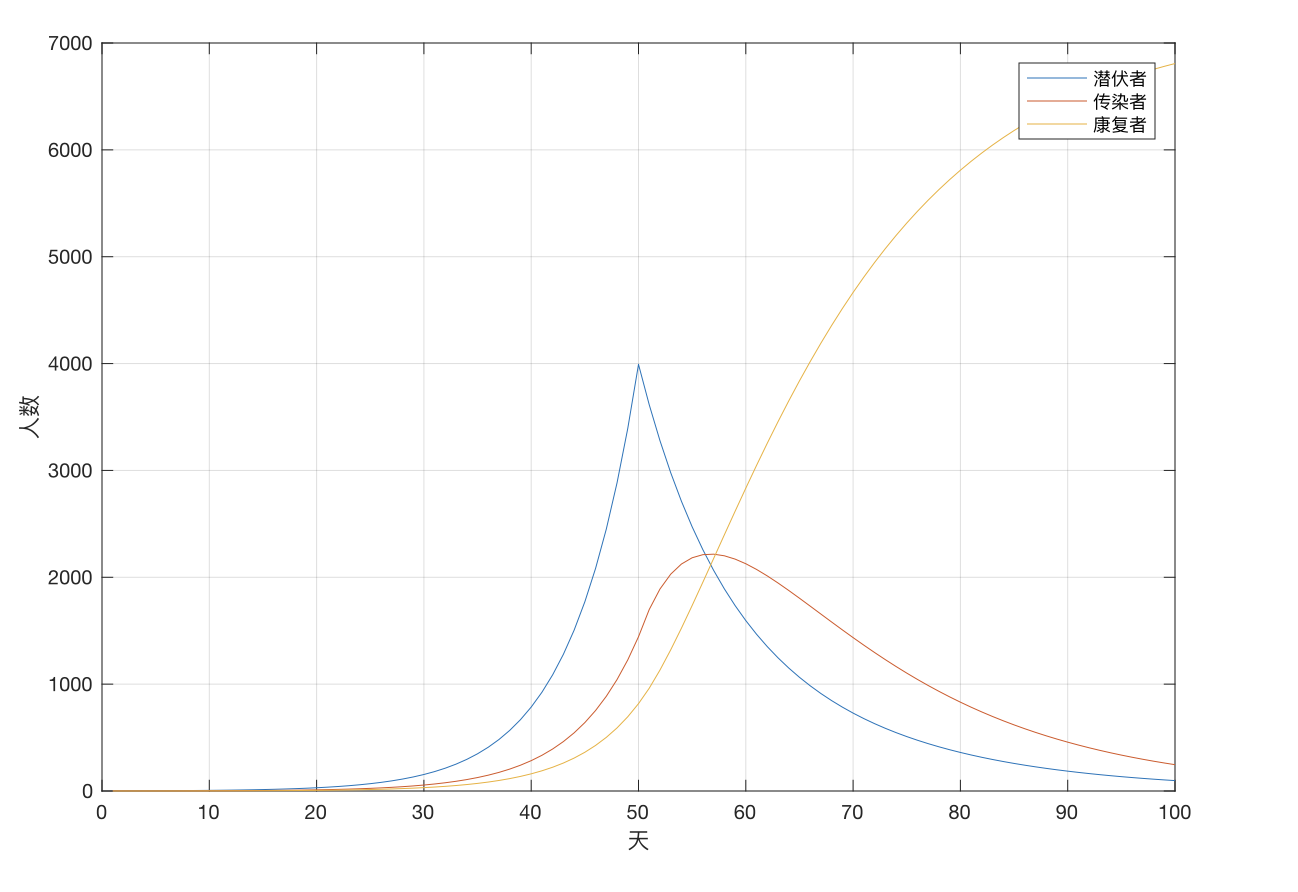
\includegraphics[width=8cm]{7.png} 
\caption{修正后的SEIR 模型的病毒传播趋势}
\end{figure}
\par
这与我们之前看到的急剧的增长曲线非常相像,
接下来我们将会针对特定参数进行调优,并与实际情况进行拟合。

\subsubsection{模型的调优与拟合}
关键参数的调整落在了感染患者(I)每天接触的易感人群的数目r、传染系数$\beta$和隔离条件上的设置上。
其中r控制着波峰的高度,$\beta$控制前期的增长坡度,隔离条件控制着下降的坡度。
\par 经过一定的调整,我们发现最合适的r为25,$\beta$为0.03,
隔离条件设置为r降到1(人)。
\par 
将图4的新增曲线离散化,还原数据集,并将其贴在图7中进行对比:
\begin{figure}[htbp][H]
\centering
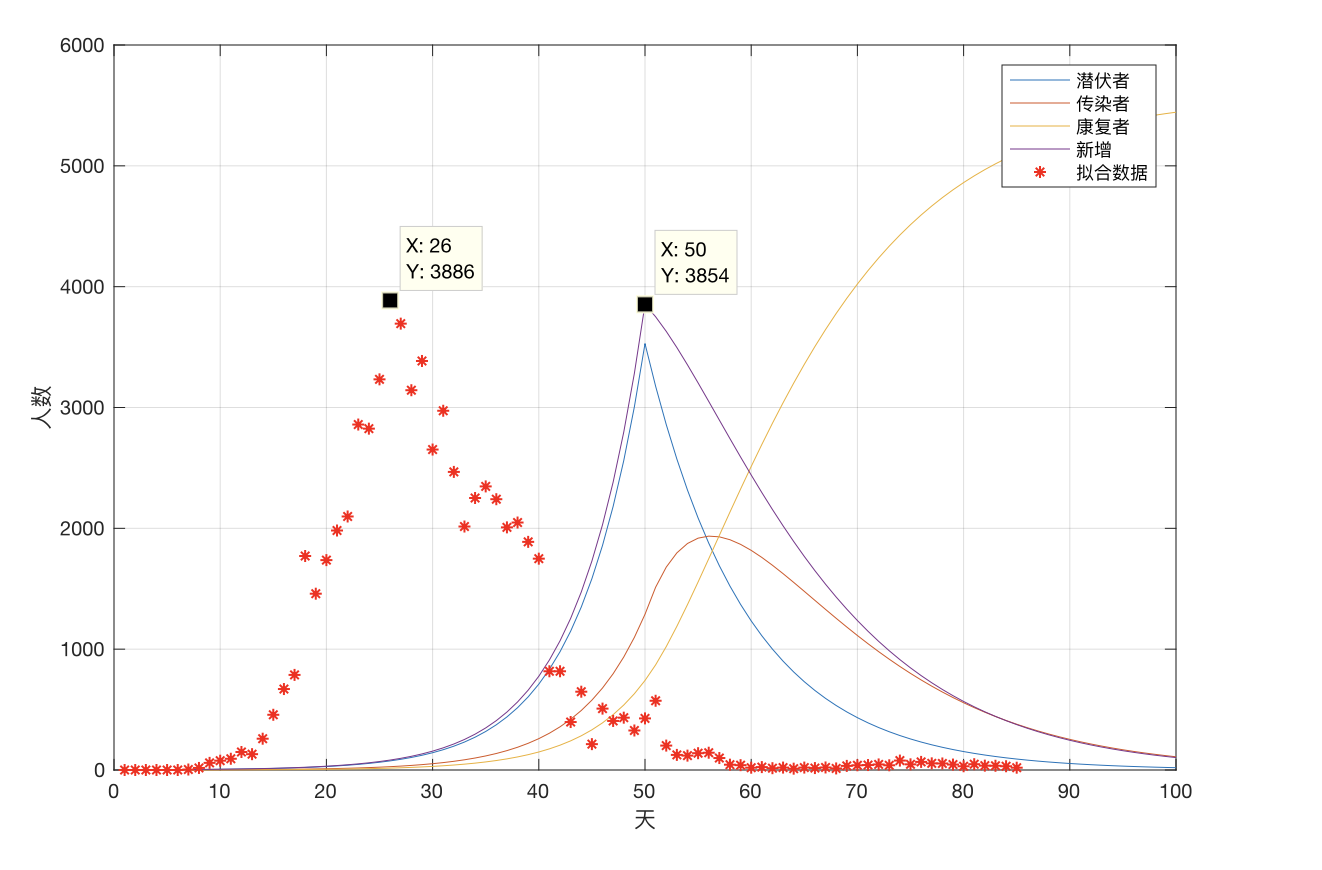
\includegraphics[width=8cm]{8.png} 
\caption{SEIR 模型的病毒传播趋势(拟合图)}
\end{figure}
\par
紫色的新增曲线是潜伏者和传染者的加权和(有未被检测可能)。
可以看到新增人数和拟合数据匹配得非常好。
同时我们可以看到两个波峰之间有一个时间差,大约是24天,
这说明疫情从刚刚开始到开始统计(1月10号)已经过去了20多天,
恰好符合疫情12月中旬开始的实际情况。
\par 
为了更好的比对数据,我们将离散数据集右移24t个单位,重新绘制曲线。

\begin{figure}[htbp][H]
\centering
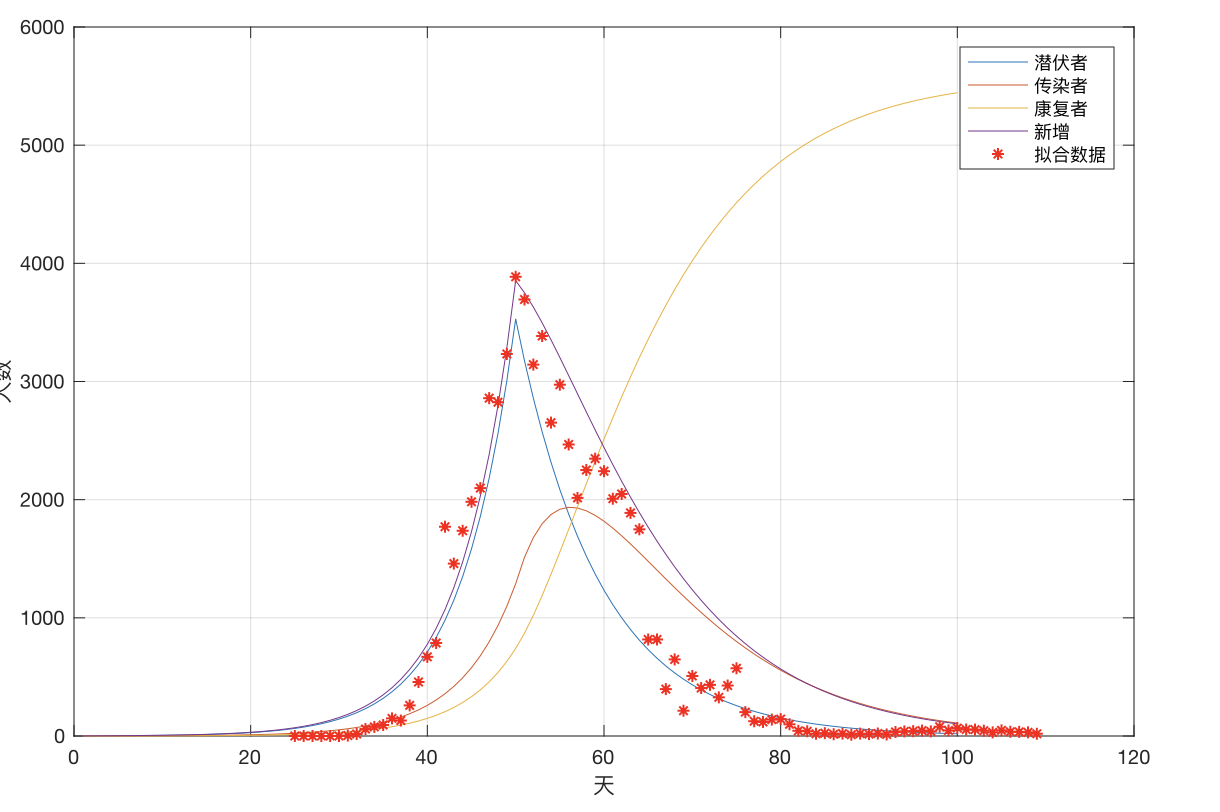
\includegraphics[width=8cm]{9.png} 
\caption{移动后的 SEIR 模型的病毒传播趋势(拟合图)}
\end{figure}
\par
可以看出,模型对疫情发展实际趋势拟合良好。


\subsection{各省新冠传播情况的分析}
\subsubsection{数据处理}
问题主要集中在各省Excel表格的数据上。
\\
\par 
由于数据全被集中到了一个表中,而Matlab的原生表格读取语句只能一次性读取一个表格的第一个工作簿,
不得不使用visual basic语言编程将表格进行了拆分。

\par 
紧接着我们发现每省的排序的顺序有问题的:部分表格被按照感染人数排序,
这样就没有办法反映出各省增长的连续情况。
我们使用人工排序的方法,将69个表格按照各省首字母进行排序。

\par 
在使用MATLAB编程时发现,
由于疫情前期部分省市数据有缺失造成矩阵维数不一致,
主要是新加入统计的省份挤占了其他省份的位置。
还有不少多报漏报的现象,我们全部进行了手工校正。


\subsubsection{数据分析}
\par 
依据34个省的69天连续统计数据,
我们绘制出去除网格的表面图如下:

\begin{figure}[htbp][H]
\centering
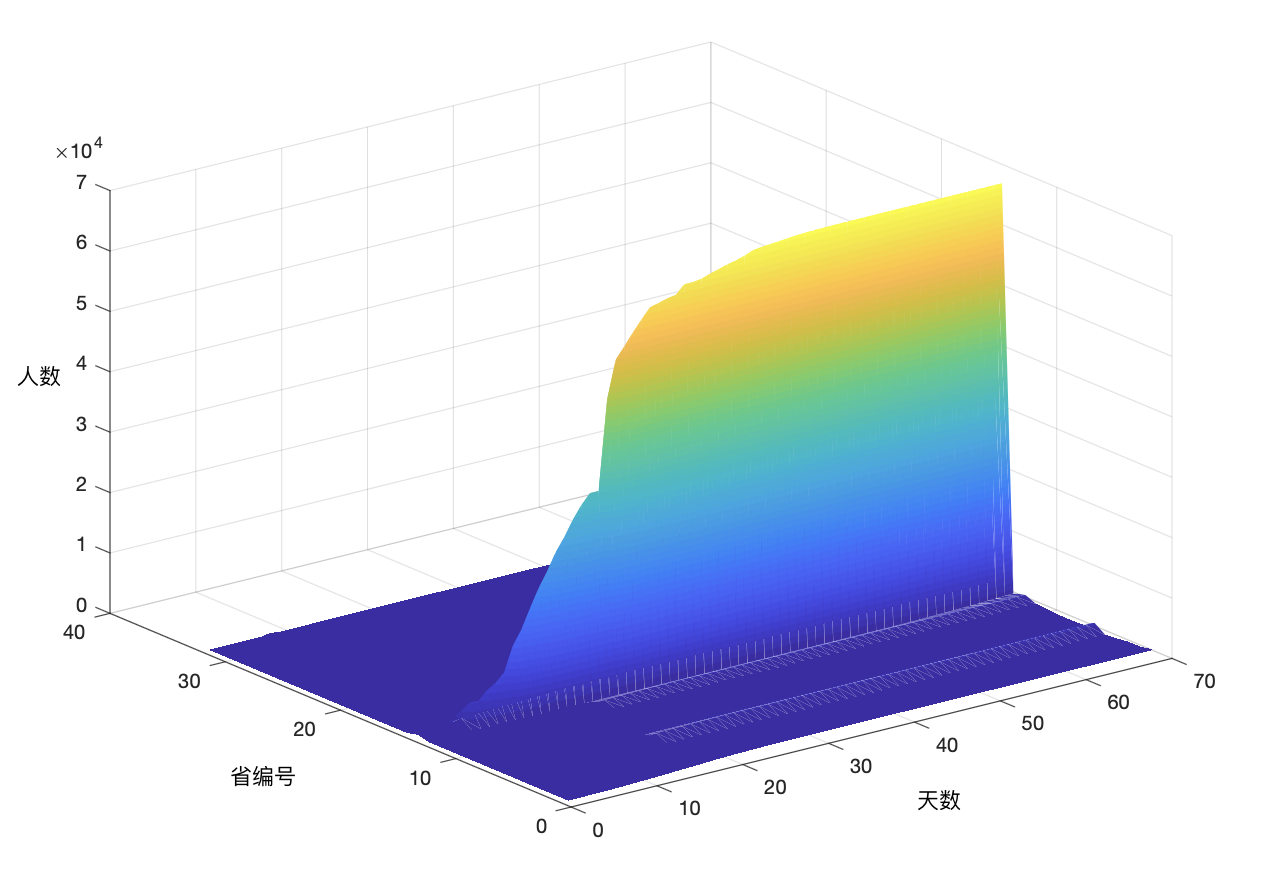
\includegraphics[width=8cm]{11.png} 
\caption{全国各省疫情发展统计图(确诊)}
\end{figure}
\par
从图10可以看出,湖北省的数据太突出,抹平了其他地区的数据差异,为了方便观察
应该去除。去除之后的统计清晰地显示了各省之间的防疫差异。

\begin{figure}[htbp]
\centering
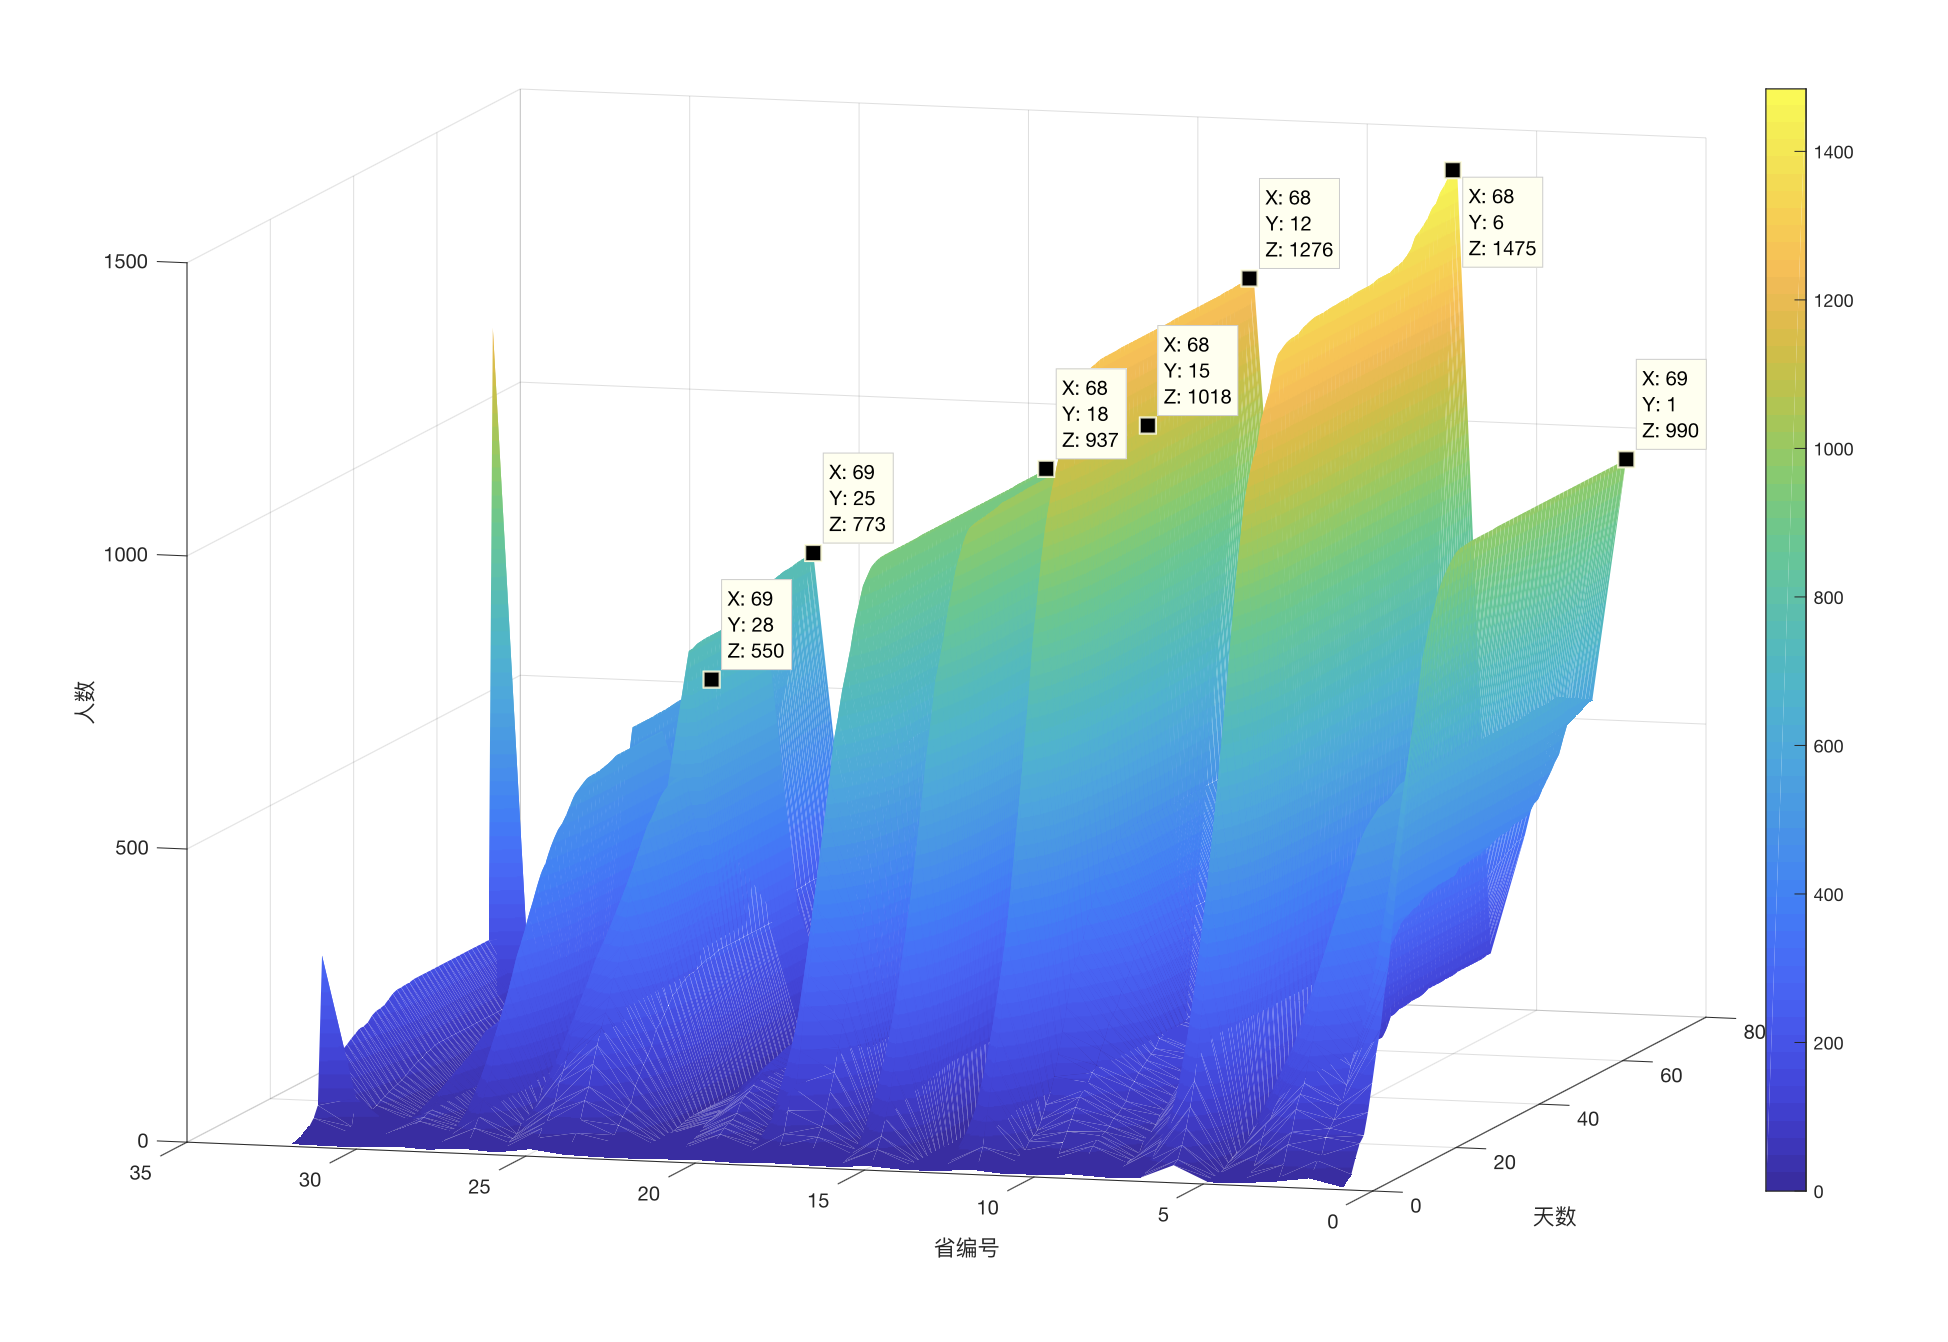
\includegraphics[width=8cm]{12.png} 
\caption{全国各省疫情发展统计图(累计确诊)}
\end{figure}
\par
各省累计确诊的增长曲线都比较相近,并不能明显地区分当地的防疫效果的优劣。
其中广东(6)与河南(12)在人数上最为突出,
广东在统计的后段还出现了疫情反扑的趋势,可能是由于港澳台和境外输入入口的缘故。除此之外各省防疫措施从结果来看都没有表现出明显差异,感染人数多少主要与人口流量和人口密度决定。

\begin{figure}[htbp][H]
\centering
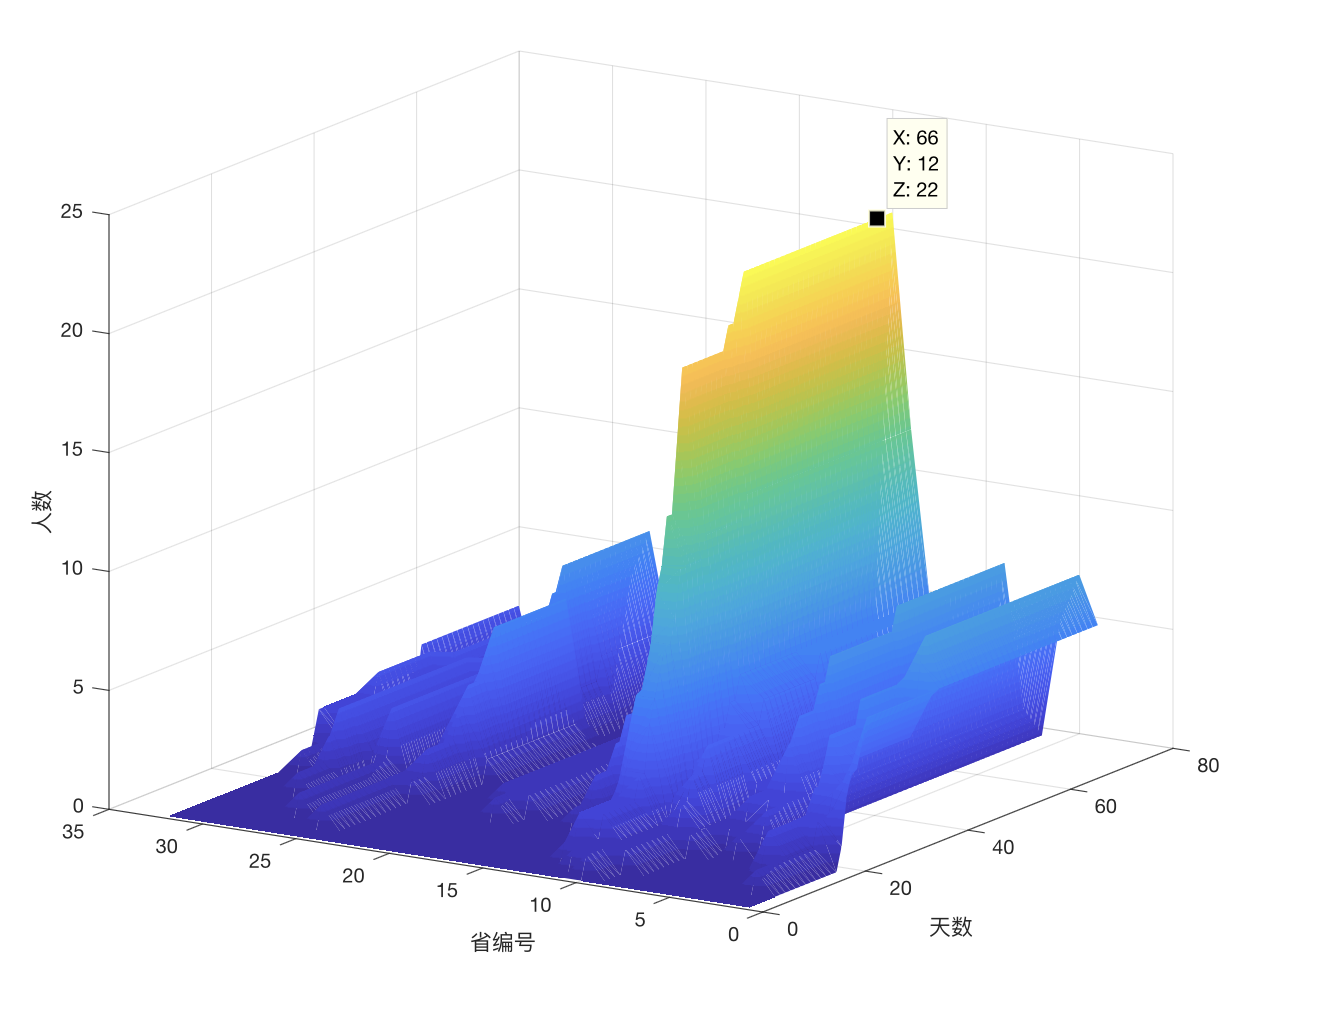
\includegraphics[width=8cm]{13.png} 
\caption{全国各省疫情发展统计图(死亡)}
\end{figure}
\par
从图12可以看出,在累计死亡人数上,河南省的数据要远远出其他省份。

\par 
有人\cite{bib3}分析认为这是由于初期感染基数较大造成的:
  \paragraph{  “河南省2020年2月16日感染确诊人数在非湖北省排名第二仅次于广东省,但是河南第一代感染基数大。
    地理位置上河南和湖北相邻,郑州又是全国交通枢纽。河南省作为一个外出务工人员大省,有很多从湖北返乡务工人员,由于湖北及全国官方通报延迟导致隔离确诊措施延迟,二代三代患者迅速生成相继发病。一代重症患者没有得到及时隔离救治,一二代轻症患者发展成重症患者造成救治困难。”
    \\\hspace*{\fill}\\
}
\par
事实上,即便是死亡人数最多的河南省也仅仅有22人,随机事件对数据影响的参数更大,并不能得出河南省防疫不力的结论。

\subsection{美国新冠病毒传播数据的统计分析}
\subsubsection{数据处理}
我们首先将dailyAmerican.xlsx 中的数据进行处理,
删去不必要的项,然后编写matlab程序(代码见附录usa.m 部分)
绘制时间序列图如下:
\begin{figure}[htbp][H]
\centering
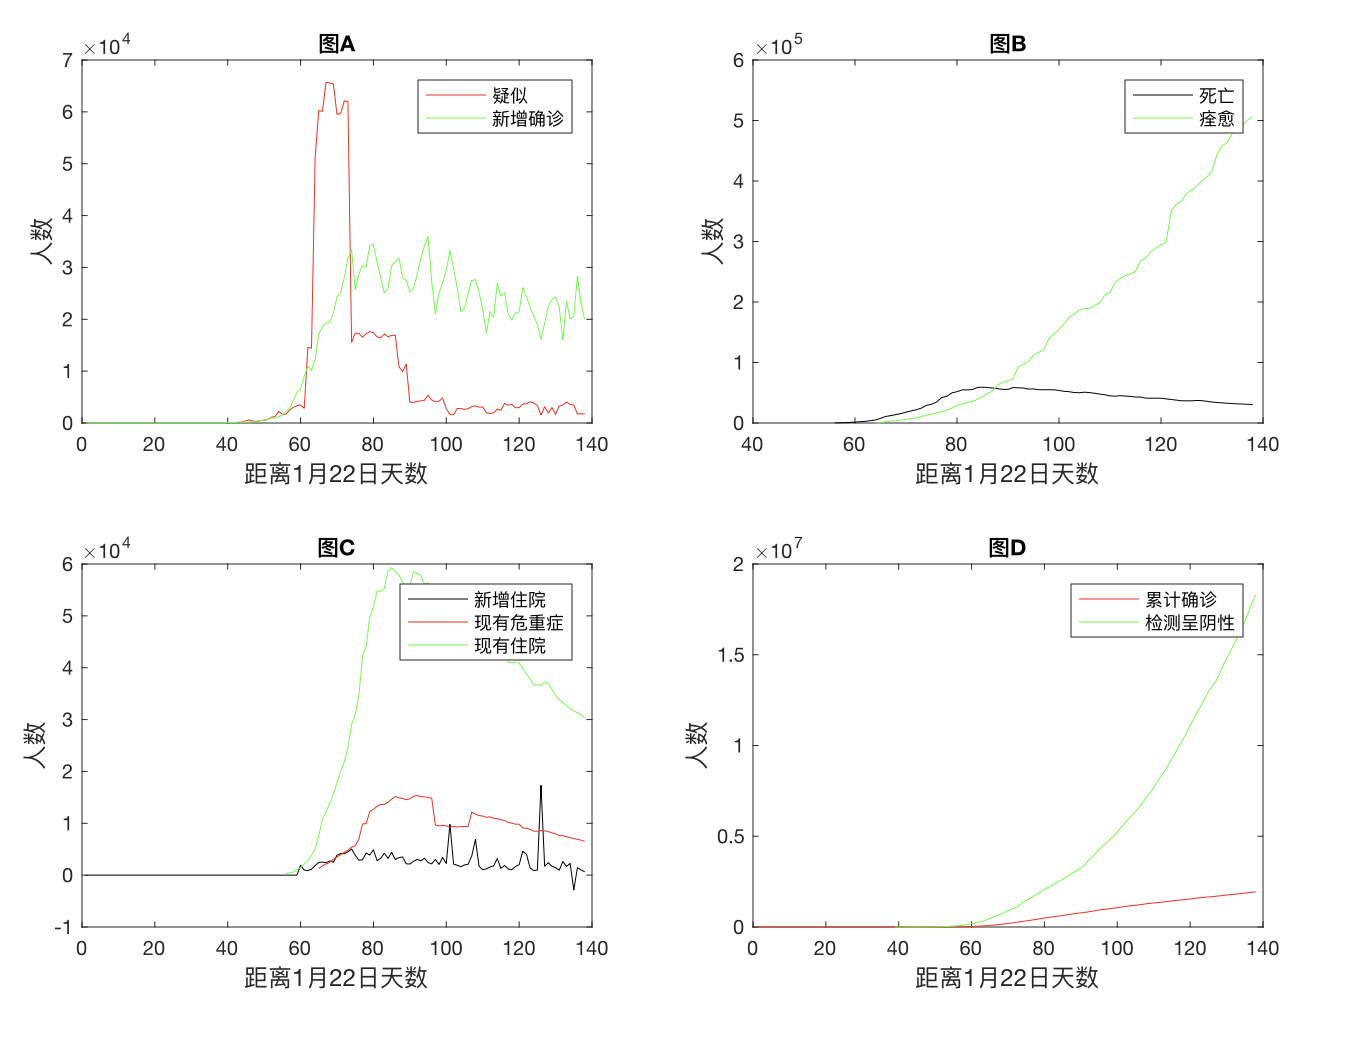
\includegraphics[width=8cm]{14.png} 
\caption{美国疫情发展统计图}
\end{figure}
\par
(由于各统计项的数量差距较大,我们将统计数据分成A、B、C、D 共4个子图呈现。)
\\
\subsubsection{数据分析} 
\par
从图A 可以看出,新增确诊人数几乎是从第50 天(3月11日)
一夜之间上涨上来的,有人认为这是美国政府在疫情前期检测量不足造成的统计误差,
但我们可以通过比对国内统计数据发现,
美国新冠病毒爆发式增长的时间恰好和图5 
中国统计境外输入病例的快速上涨时间重合。
鉴于此时的中国已经建立了较为完善的病毒检测体系,因此这种说法是不准确的。
\\
\par
从全部A、B、C、D四张图中都可以发现病毒传播速度在第60天(3月21日)的增长达到了高峰,
到第80天增长到达极限,该过程一共20天左右,这恰好和图4中中国疫情发展时间相同。之后美国新冠病毒新增数据趋于稳定,而住院、死亡人数开始逐渐下降。
\\
\par
但值得注意的是,与图4、5中国疫情发展趋势相比,图A显示的每日新增人数在到达高峰之后并没有快速下降,而是在高位不断波动。根据我们在美疾控制中心\cite{usaCdc}得到的后续疫情发展数据,直到六月末,疫情不仅没能够快速得到遏制,反而在有了抬头的趋势(见图14)
\\

\begin{figure}[htbp][H]
\centering
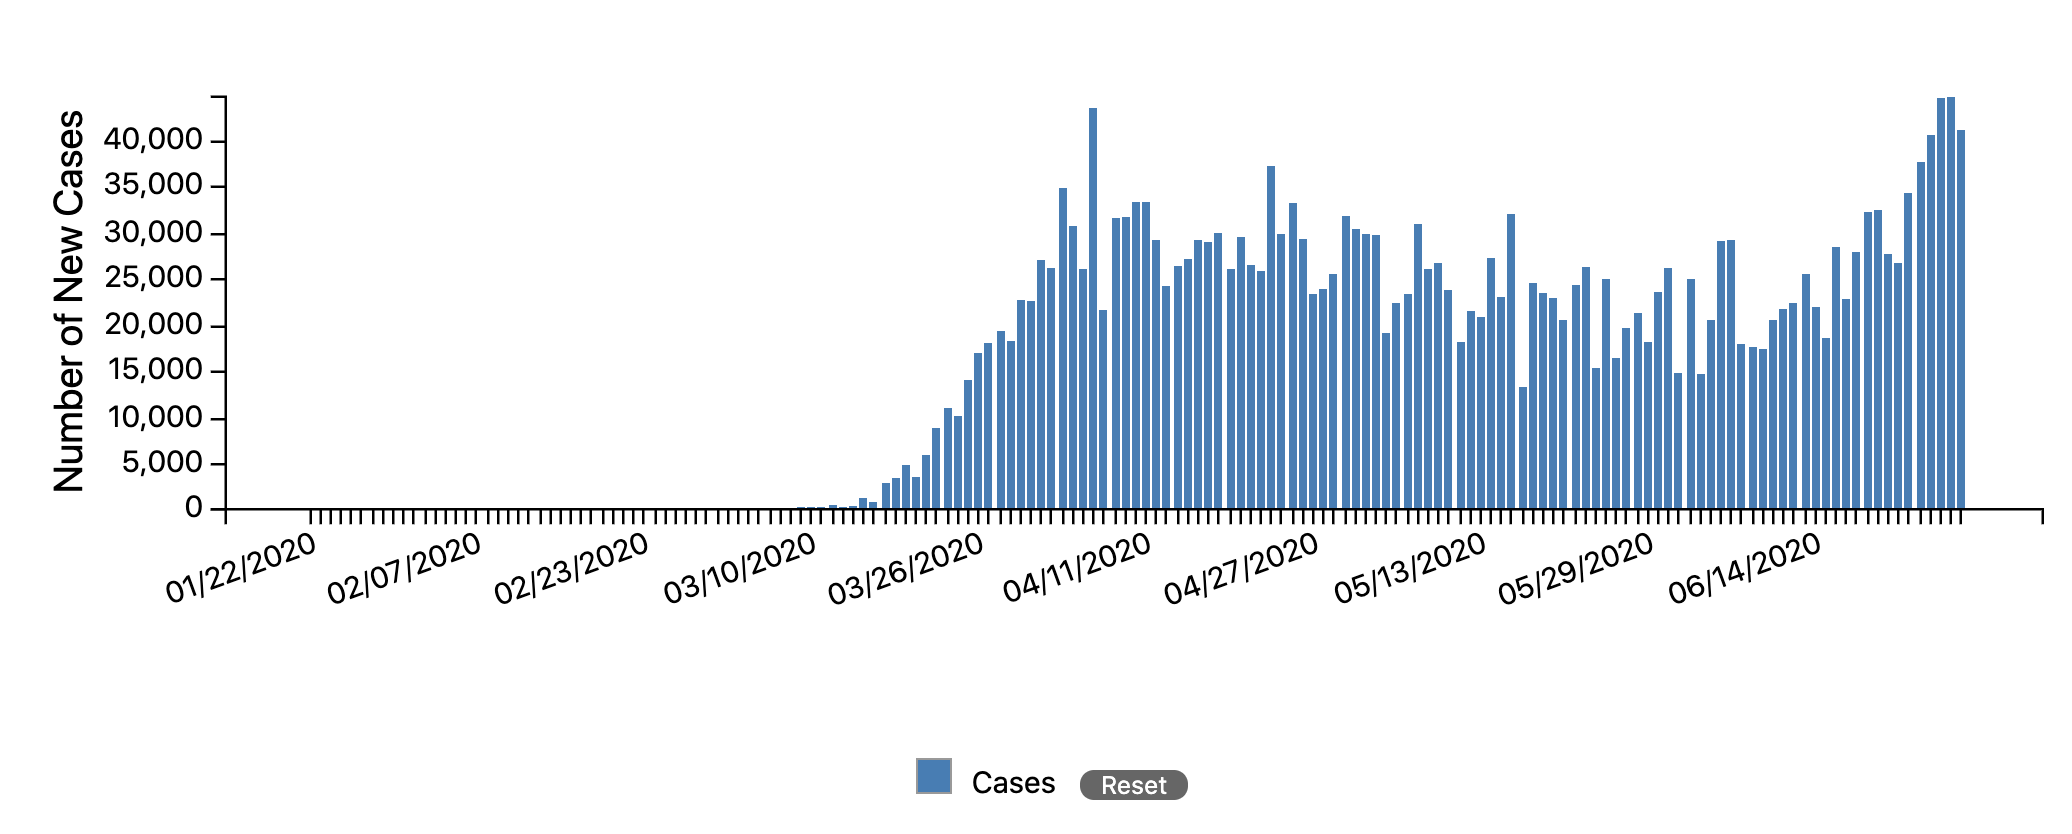
\includegraphics[width=8cm]{caseIncrease.png} 
\caption{美疾控中心每日新增数据}
\end{figure}
\par

对于这一现象,哥伦比亚大学梅尔曼公共卫生学院环境卫生科学系发表的论文\textit{Projection of COVID-19 Cases and Deaths in the US as Individual States Re-open May 4, 2020
}\cite{papercdc}是这么解释的:
\par
\paragraph{
"In March and April 2020, 
control measures enforcing social distancing and 
restricting individual movement and contact were 
adopted across the United States in an effort to 
slow the spread and growth of COVID-19. However, 
a number of states have now begun to ease these restrictions."\cite{papercdc} }
\par
可见,在疫情后半段显示出的两国病毒传播的发展趋势上的差异是由两国不同的防疫措施引起的:美国部分州在疫情还没能得到控制的情况下贸然解封,导致新增感染人数重新上升。\\

\par 
我们通过美疾控中心官网和纽约时报\cite{nyt}相关报道可以找到美复工和停摆的州的动态图(图15),通过比对可以发现,疫情高发州在短暂复工后又纷纷重新开始施行隔离措施。

\begin{figure}[htbp][H]
\centering
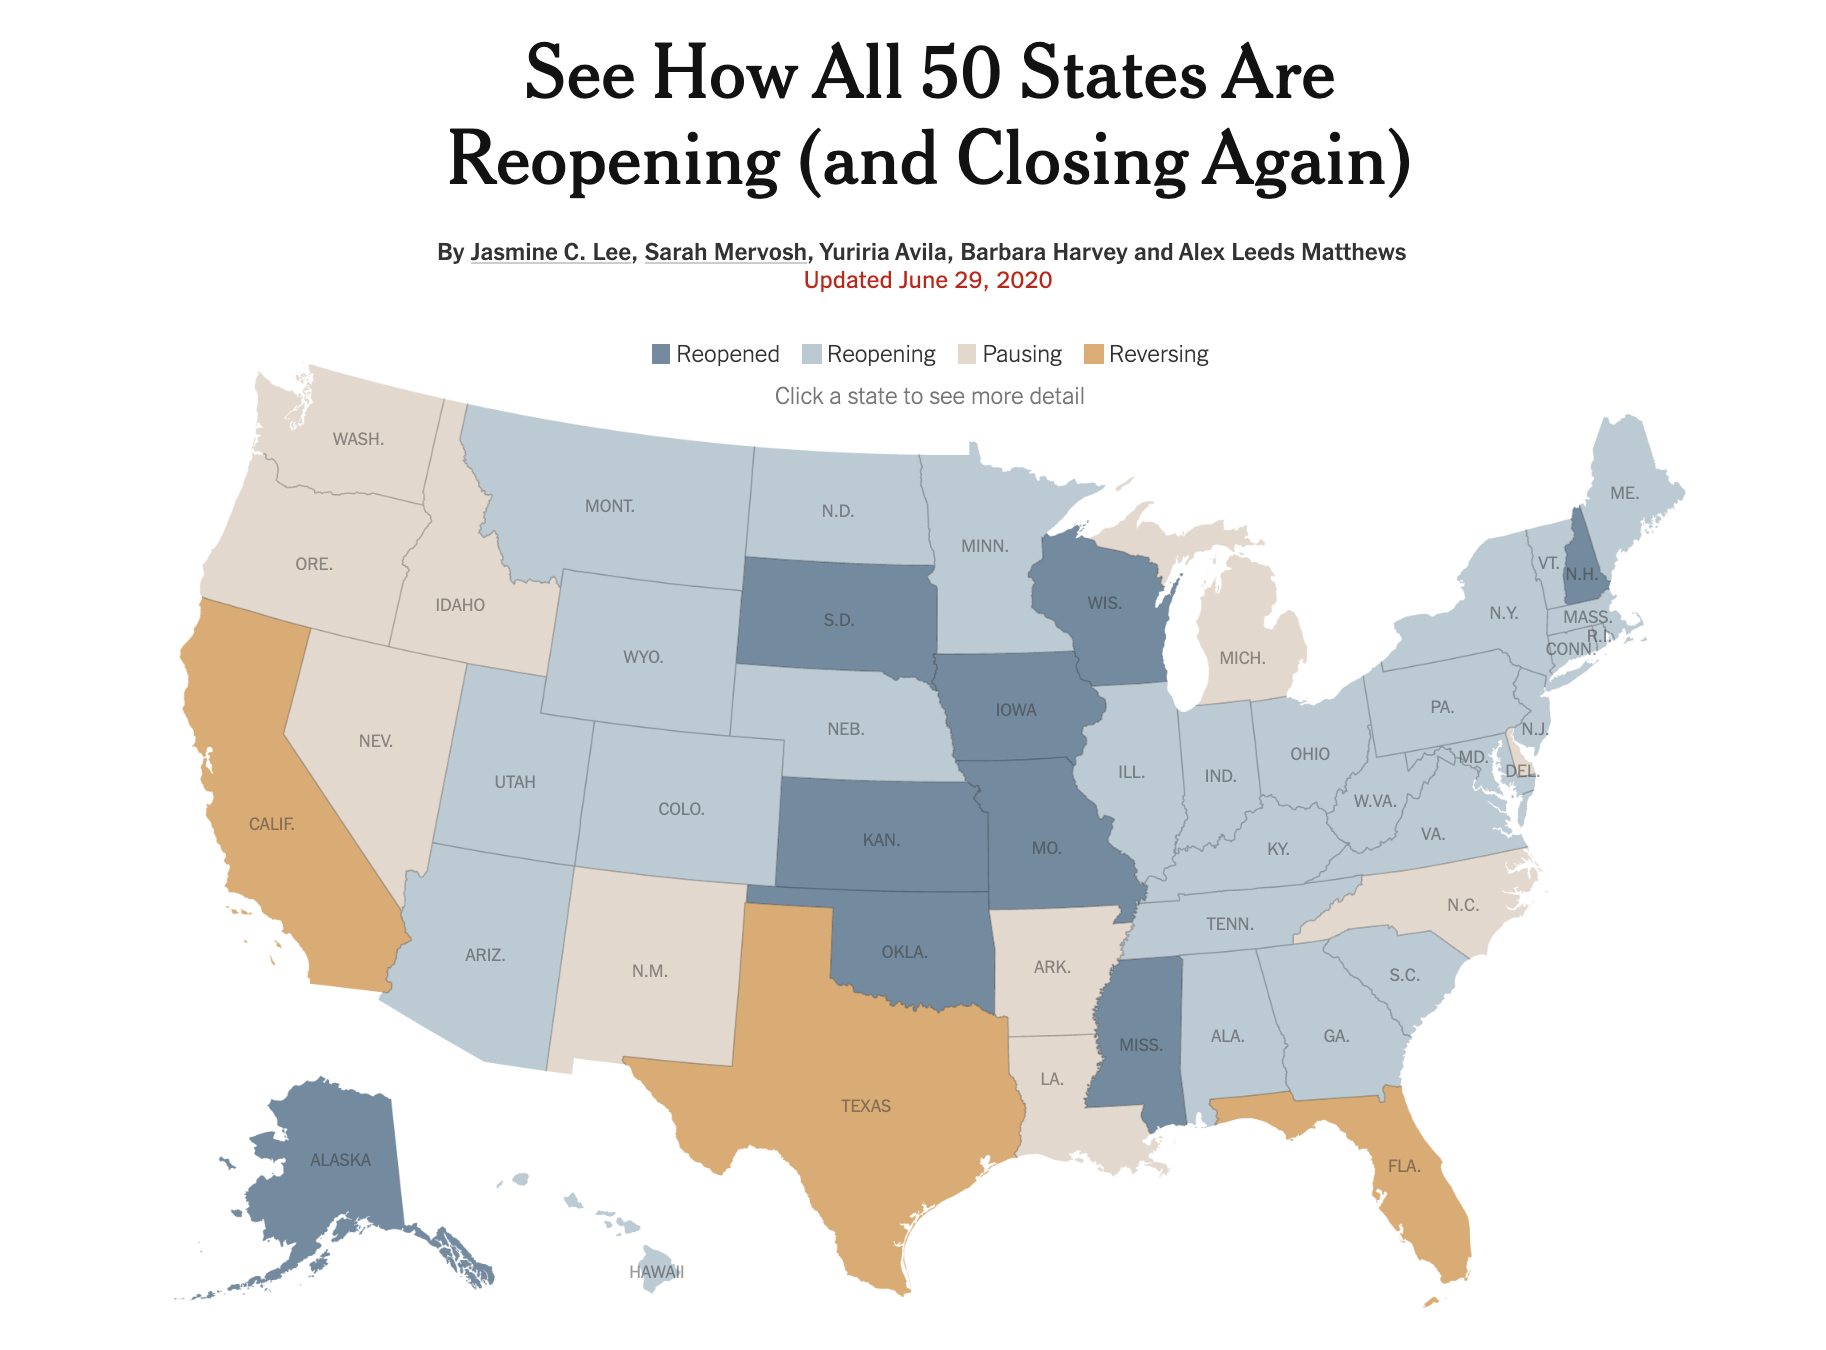
\includegraphics[width=8cm]{nyt.png} 
\caption{纽约时报:复工后又再度关闭的州}
\end{figure}
\par


\subsection{美国新冠病毒传播的预测}


\subsubsection{元胞自动机模型的描述}
\par
由于美国疫情主要发生在纽约等大城市中,
人员密集度高,而封锁又不彻底,病毒传播因素变化大。
传统的病毒感染模型并不能很好的模拟这一动态情况。
所以我们选择了元胞自动机模型来模拟美国疫情的传播情况。
\\

    \par
细胞自动机(英语:Cellular automaton),
又称格状自动机、元胞自动机,是一种离散模型,
在可计算性理论、数学及理论生物学都有相关研究。
\par 
它是由无限个有规律、坚硬的方格组成,
每格均处于一种有限状态。整个格网可以是任何有限维的。
同时也是离散的。每格于t时的态由t-1时的一集有限格(这集叫那格的邻域)的态决定。
每一格的“邻居”都是已被固定的。(一格可以是自己的邻居。)
每次演进时,每格均遵从同一规矩一齐演进。\cite{bib4}\\
\par 
标准的元胞自动机(A)由元胞、元胞状态、
邻域和状态更新规则构成。数学表示为\cite{bib5}。
$$A=(L,D,S,N_1,f)$$
\par 
其中L为元胞空间;d为元胞自动机内元胞空间的维数;
S是元胞有限的、离散的状态集合;$N_1$为某个邻域内所有元胞的集合;
f为局部映射或局部规则。
元胞空间是元胞所分布的空间网点的集合。
理论上元胞空间在各个维向上是无限延伸的,为了能够在计算机上实现,
而定义了边界条件,包括周期型、反射型和定值型\cite{bib6}。
一个元胞通常在一个时刻只能取自一个有限集合的一种状态,
例如{0,1}。元胞状态可以代表个体的态度,特征,行为等[7]。
在空间上与元胞相邻的细胞称为邻元,所有邻元组成邻域。
\\
\par
元胞自动机的一大魅力在于,尽管它本身的理论描述有着近乎唬人的复杂度,
但它的实现却是非常简单直观的,它给了建模者相当大的自由度来决定模型的实现,从最简单的用来演示的生命游戏,到妄图解释整个宇宙运行规则的万物理论\cite{wol}
\\
\par


\subsubsection{模型实现}

我们依据元胞自动机原理编写了matlab程序(代码见附录map.m 部分)
我们将初始元胞大小设置为美国人口(截至2019年1月为3.3亿\cite{bib8})
的1/1000 ,单位长为$575=\sqrt{33000}$。
\\
\par 
为了简化模型,我们设置了两个元胞动态参数:人群感染概率(getInfected)和人员流动密度(peopleInGrowth),初始值分别为0.06和0.005。分别由一个575$\times$575的伪随机矩阵分发。
\par
元胞自动机的维数为3,第零层为R人群(removed)用黑色表示,第一层为I人群(infected)用红色表示,第二层为S人群(susceptible) 用绿色表示。为了使模型模拟过程直观,我们采用了MVC设计模式将业务逻辑、数据和界面显示分离,将元胞矩阵的动态更新分别映射到一个平面像素图和一个折线图上,并实时刷新数据(图16、17)。
\\ 
\begin{figure}[htbp]
    \centering
    \begin{minipage}[t]{0.48\textwidth}
    \centering
    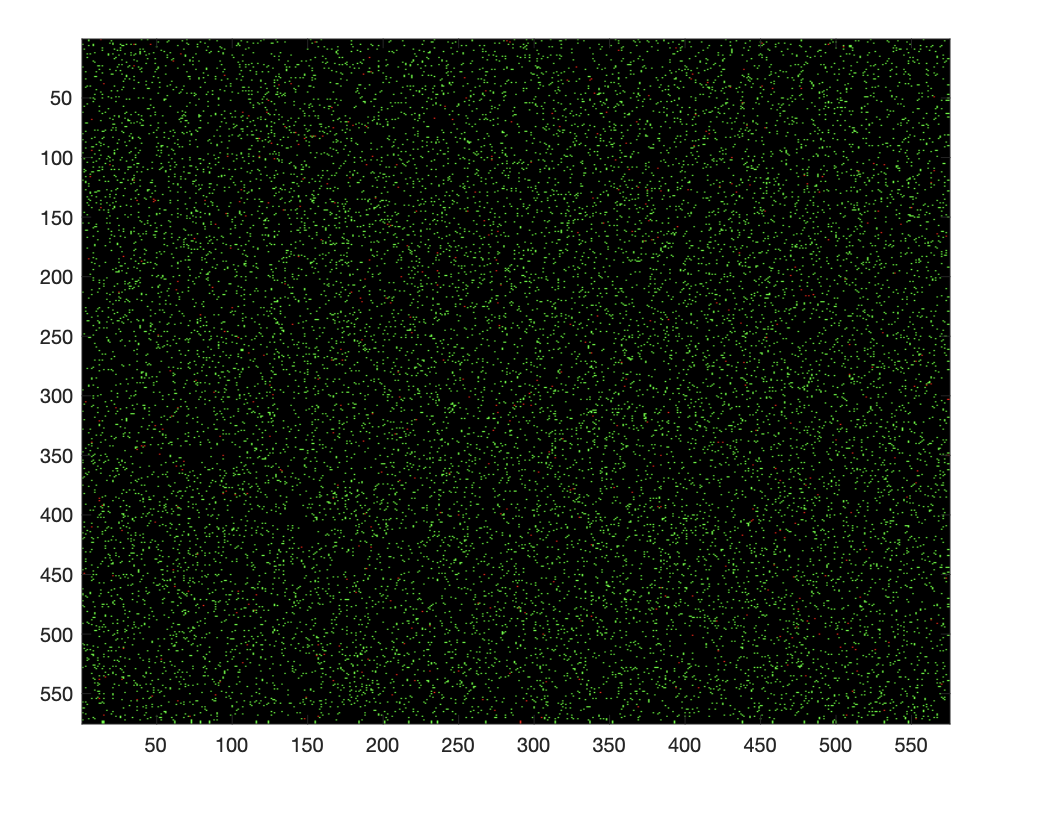
\includegraphics[width=6cm]{20.png}
    \caption{元胞自动机模拟图}
    \end{minipage}
    \begin{minipage}[t]{0.48\textwidth}
    \centering
    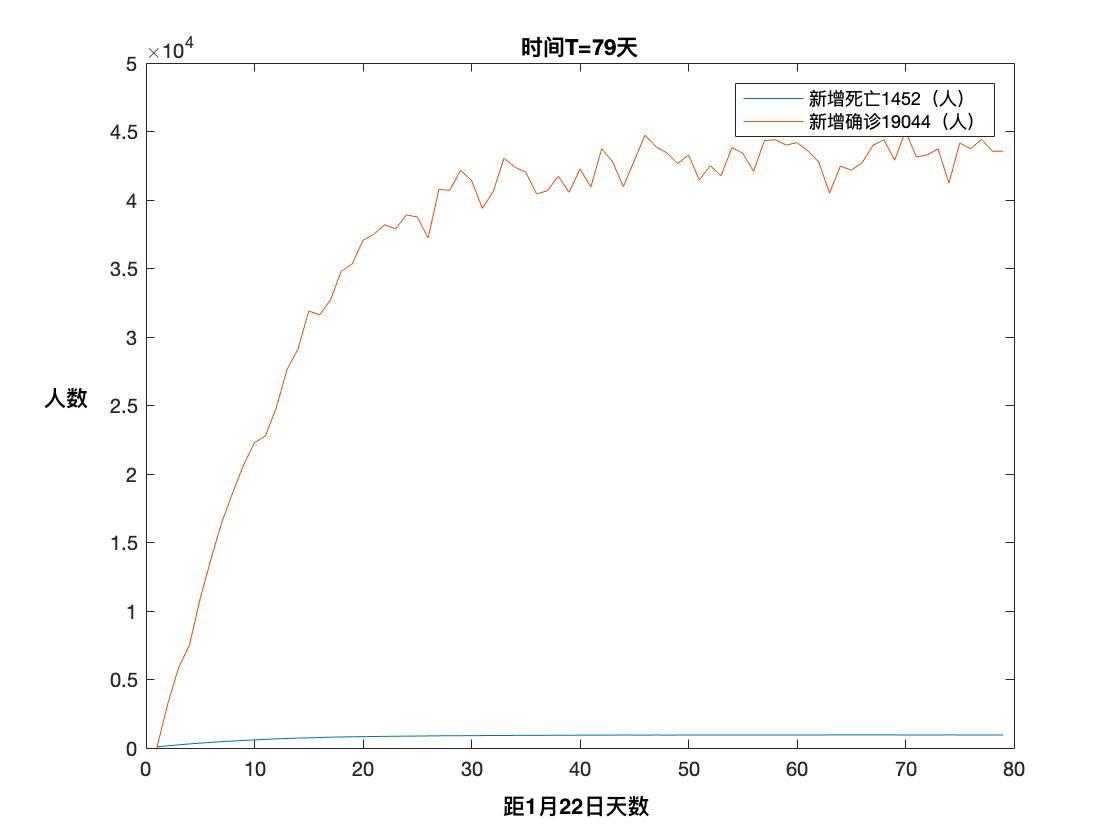
\includegraphics[width=6cm]{raw.jpg}
    \caption{元胞自动机折线动态图}
    \end{minipage}
    \end{figure}
\subsubsection{模型的调优与拟合}
\par 
静态的元胞参数显然没法反映变化多端的美国新冠疫情数据变化情况。为此,我们基于现实的美国新冠疫情数据对人群感染概率(getInfected)和人员流动密度(peopleInGrowth)两个参数进行了动态调优。重绘后的折线图和实际数据拟合如下(图18)
\begin{figure}[htbp][H]
\centering
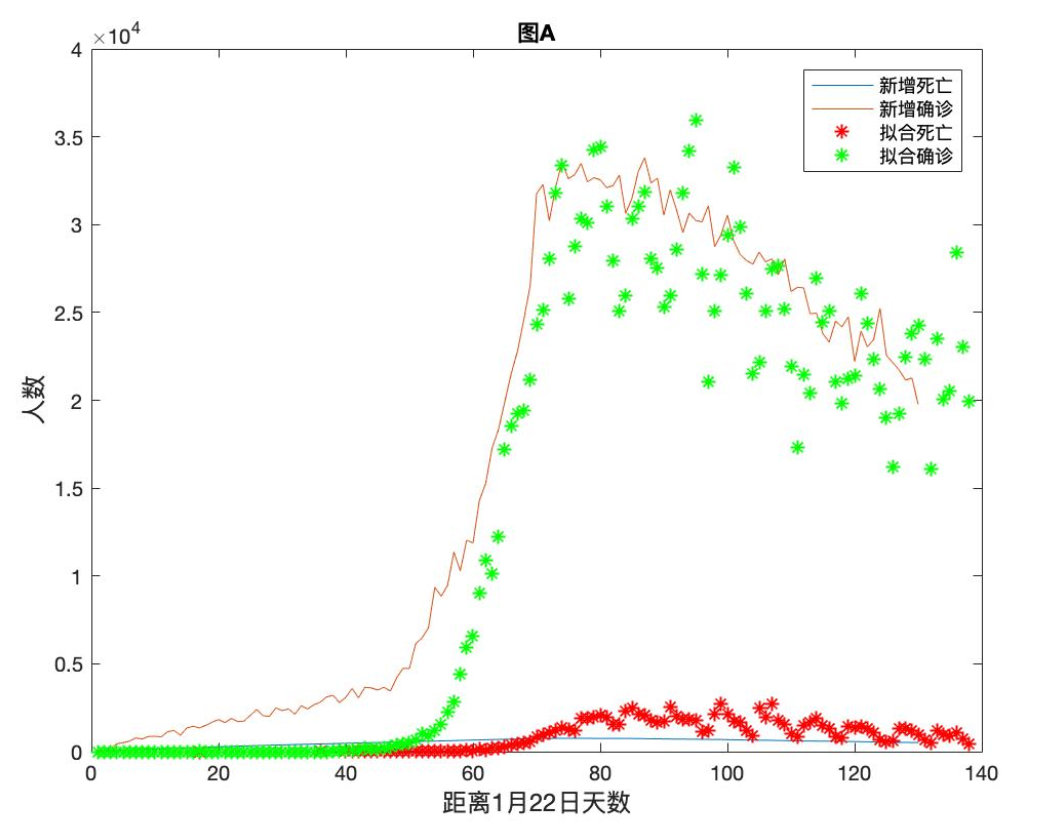
\includegraphics[width=8cm]{sim.png} 
\caption{元胞自动机折线拟合图}
\end{figure}
\par
可以看出模型在后半段对疫情发展实际趋势拟合良好,因此我们将元胞更新的时间周期延长至于160天(6月30日)重新模拟来预测美国六月的疫情发展情况。
\begin{figure}[htbp][H]
\centering
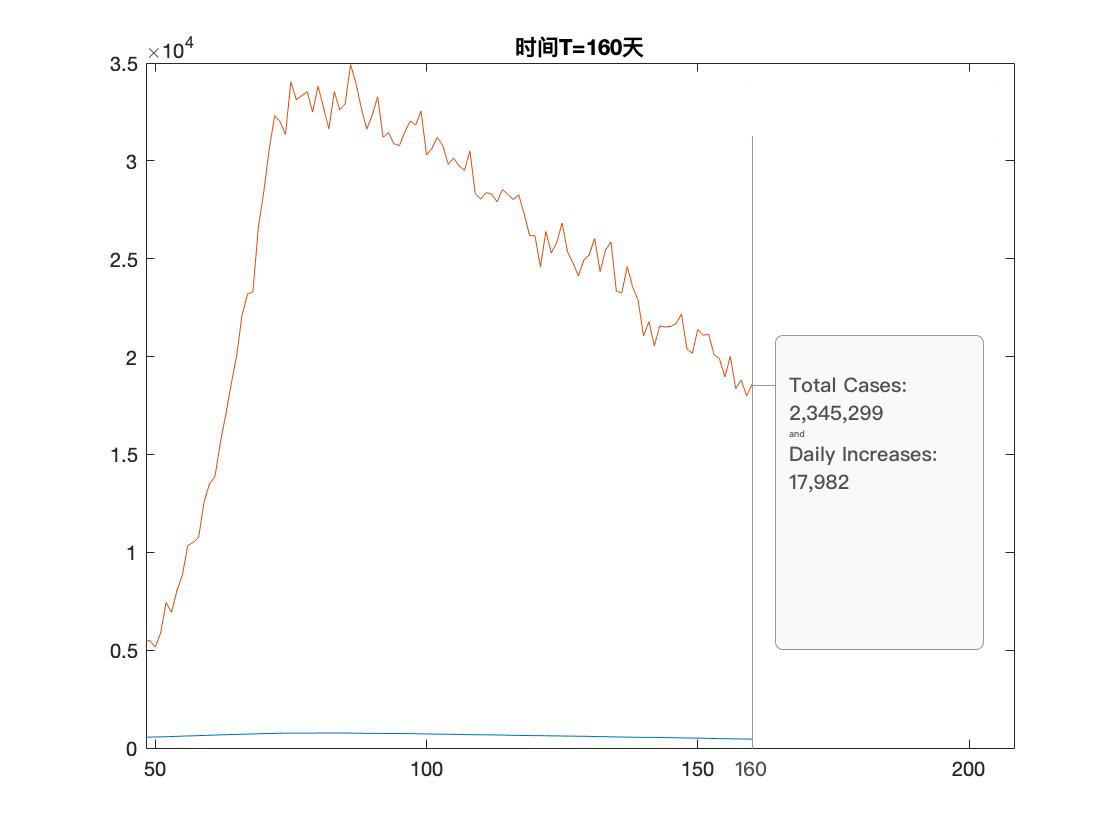
\includegraphics[width=8cm]{presim.png} 
\caption{美国疫情数据预测}
\end{figure}
\par
模拟结果显示,在我们的模型中新增确诊人数会在六月末逐渐下降,死亡人数则保持稳定。
数据经过累加我们预测美国六月份感染总人数会达到2,345,299人。(图19)
\\
\par
然而在本文写作的同时,六月份逐渐过去,现实情况却与我们预料的有所不同。

\section{模型评价\&改进}
\par 
现实情况与我们预测的大相径庭,美国疫情进入六月末之后感染人数快速上升,不久就突破了250万,多个州在重启之后再度封锁……
\par
这不禁让人想起伯兰特·罗素著名的火鸡问题:火鸡中的一个科学家经过一年的不断观察,发现农场主每天早上11点的时候会给它们投饲料,于是在感恩节这一天它宣布了自己这个伟大发现。但是早上11点过去,农场主并没有来投饲料,反而带了一把枪把它们全杀了。
\par 
火鸡问题多多少少反映出了归纳主义者的困境。“过去的未来和未来的未来是否相似”这个问题不能由过去的经验解决,只有等未来已来时才能得到验证,但很多人误以为验证得来的结论就是真理,有的时候这不过是一种侥幸罢了。
\par 
在这个数学模型中。我们原以为增加伪随机函数分发的元素,可以在虚假的随机中找出不由随机事件变化的规律。但事实上世界的发展是可能是由无限不可列多个参数决定的(当然,这是一种陈旧的机械决定论的想法),谁也不知道未来会发生什么。基于过去的假设,通常在未来的突变来临时不堪一击。
\par
现在人工智能和大数据的概念被媒体和金融投机者炒得火热,很多不知情的外行人把它吹捧成无所不能的万金油。事实上,所谓的人工智能和”智能“这个概念还相差很远,倒是和中世纪的炼金术很相像:将参数的设置和拟合过程由大量计算黑箱自动求解,通过已有的数据训练出针对未来情形的通用解决公式。这在客观条件变化有限的应用场景已经取得了突破性的进展,例如围棋和识别文字,但在更加复杂的情形却注定是无所作为的,原因就在于计算机不能理解无限,它所能做的只不过是用有限的位运算来笨拙的模拟无限的概念。
\\
\par 
回到本模型上,由于编程人员的懒惰,大多数结论性的评价没有通过统计学的计算语言表达,而仅仅通过直观反映。这是本文最需要改进的地方,但是由于三位作者的统计学水平近乎文盲,直到写作完成这个问题也未能得到解决,成了一个不小的遗憾。
\par
在附录里,您很容易发现源代码混乱不堪,Debug处理和多功能的注释混杂在一起。尽管我们打算在编写附录时重新整理代码,但是您依然可能发现在您的计算机中无法正常运行文中展示的全部功能。
\par 
本文的写作者在中途因为不堪忍受word在处理中型文档时的频繁卡顿和崩溃,将写作环境迁移到了\LaTeX 上。因此论文格式的规范可能是本文为数不多的一个优点,但这完全不是我们的功劳。
\par 
在参数的拟合上,特别是元胞自动机参数的动态拟合上。原本打算采用CoreML中较为成熟的机器学习框架实现,但是由于本文的案例较为简单,而CoreML的API文档时着实较为复杂。最后改成了单位花费最小的人工实现,希望能在以后的学习中掌握更多对数据进行操作的工具和方法,写出一篇真正像样的论文。
\\
\par 
(完)

\newpage


\begin{thebibliography}{66}
    \bibitem{bib1}
    https://github.com/BlankerL/DXY-COVID-19-Data
    \bibitem{bib2}
    https://web.phb123.com/city/renkou/city\_241.html?ivk\_sa=1023345q 
    \bibitem{bib3}
    https://www.zhihu.com/question/372225552/answer/1019781435
    \bibitem{bib4}
    https://w.upupming.site/wiki/元胞自动机
    \bibitem{bib5}
    S. Amoroso; Y.N. Patt. Decision procedures for surjectivity and injectivity of parallel maps for tessellation structures. Journal of Computer and System Sciences. October 1972
    \bibitem{bib6}
    周成虎; 孙战利 谢一春. 地理元胞自动机研究. 北京: 科学出版社. 2000: 26–51. ISBN 9787030081209.
    \bibitem{bib7}
    Wolfram 2002,第231页
    \bibitem{bib8}
    https://w.upupming.site/wiki/美国
    \bibitem{nyt}
    https://www.nytimes.com/interactive/2020/us/states-reopen-map-coronavirus.html
    \bibitem{usaCdc}
    https://www.cdc.gov/coronavirus/2019-ncov/covid-data/covidview/index.html
    \bibitem{papercdc}
    Teresa Yamana; Sen Pei; Sasikiran Kandula; Jeffrey. Department of Environmental Health Sciences, Mailman School of Public Health,
    Columbia University. ShamanProjection of COVID-19 Cases and Deaths in the US as Individual States Re-open May 4, 2020
    \bibitem{wol}
    https://www.wolframphysics.org/technical-introduction/potential-relation-to-physics/
    \end{thebibliography}

\newpage
\section{附录}
\subsection{声明}
\par 
本文的git本地仓库由于体积原因已于写作完成之时全部从本机移除,但是您还可以通过访问该仓库在GitHub上的备份:
\\ 
https://github.com/Gaochengzhi/math\_module\_task 
\\ 来获取全部的文档、源代码、图片和表格。

\subsection{domestic.m}
\lstset{
    breaklines=true,  %代码过长则换行
    numbers=left, %行号在左侧显示
    numberstyle= \small,%行号字体
    keywordstyle= \color{blue},%关键字颜色
    commentstyle=\color{gray}, %注释颜色
}
\begin{lstlisting}
    clc; clear; close all;
    % 中国感染数据处理
    [data, text] = xlsread('meta.xlsx');
    total = data(:, 2);
    increased = data(:, 3);
    infectedNow = data(:, 4);
    death = data(:, 5);
    cure = data(:, 6);
    HMT = data(:, 10);
    abroad = data(:, 11);
    x = [1:85];
    % 修正数据前
    figure(1);
    plot(x, total, 'k:', x, infectedNow, 'r', x, cure, 'g');
    xlabel('距离1月10日天数', 'Fontsize', 12);
    ylabel('人数', 'Fontsize', 12);
    title('中国新冠疫情发展85天趋势(总数,现有感染者,治愈数)', 'Fontsize', 16)
    legend('total', 'infectedNow', 'cure');
    figure(2)
    plot(x, increased, 'b', x, death, 'k', x, HMT, 'k.-', x, abroad, 'c--');
    xlabel('距离1月10日天数', 'Fontsize', 12);
    ylabel('人数', 'Fontsize', 12);
    title('中国新冠疫情发展85天趋势(新增,死亡,港澳台,境外输入)', 'Fontsize', 16)
    legend('increased', 'death', 'HMT', 'abroad');
    % 修正数据后
    [data, text] = xlsread('remeta.xlsx');
    total = data(:, 2);
    increased = data(:, 3);
    infectedNow = data(:, 4);
    death = data(:, 5);
    cure = data(:, 6);
    HMT = data(:, 10);
    abroad = data(:, 11);
    x = [1:85];
    figure(3);
    plot(x, total, 'k:', x, infectedNow, 'r', x, cure, 'g');
    xlabel('距离1月10日天数', 'Fontsize', 12);
    ylabel('人数', 'Fontsize', 12);
    title('处理后的中国新冠疫情发展85天趋势(总数,现有感染者,治愈数)', 'Fontsize', 16)
    legend('total', 'infectedNow', 'cure');
    figure(4)
    plot(x, increased, 'b', x, death, 'k', x, HMT, 'k.-', x, abroad, 'c--');
    xlabel('距离1月10日天数', 'Fontsize', 12);
    ylabel('人数', 'Fontsize', 12);
    title('处理后的中国新冠疫情发展85天趋势(新增,死亡,港澳台,境外输入)', 'Fontsize', 16)
    legend('increased', 'death', 'HMT', 'abroad');
\end{lstlisting}
\newpage
\subsection{read.m}
\begin{lstlisting}
    clc; clear; close all;
    files = dir('Provice/*.xlsx');
    countNumber = [];
    x = [1:69];
    y = [1:32];
    [xx, yy] = meshgrid(x, y);
    
    for index = 1:69
        filename = files(index).name;
        index = num2str(index);
        name = strcat('Provice/', index, '.xlsx');
    
        %    name = strcat('Provice/', filename);
        [data, text] = xlsread(name);
        countNumber = [countNumber, data(1:32, 1)];
        z = countNumber;
    end
    figure(1)
    surf(xx, yy, z)
    shading interp;
    xlabel('天数');
    ylabel('省编号');
    zlabel('人数');
    %去除武汉
    countNumber = [];
    x = [1:69];
    y = [1:32];
    [xx, yy] = meshgrid(x, y);
    for index = 1:69
        filename = files(index).name;
        index = num2str(index);
        name = strcat('Provice/', index, '.xlsx');
        [data, text] = xlsread(name);
        countNumber = [countNumber, data(1:32, 1)];
        z = countNumber;
    end
    z(14, :) = 0;
    figure(2)
    surf(xx, yy, z)
    shading interp;
    xlabel('天数');
    ylabel('省编号');
    zlabel('人数');
    %死亡
    countNumber = [];
    x = [1:69];
    y = [1:32];
    [xx, yy] = meshgrid(x, y);
    for index = 1:69
        filename = files(index).name;
        index = num2str(index);
        name = strcat('Provice/', index, '.xlsx');
    
        %    name = strcat('Provice/', filename);
        [data, text] = xlsread(name);
        countNumber = [countNumber, data(1:32, 2)];
        z = countNumber;
    end
    z(14, :) = 0;
    figure(3)
    surf(xx, yy, z)
    shading interp;
    xlabel('天数');
    ylabel('省编号');
    zlabel('人数');
    %康复
    countNumber = [];
    x = [1:69];
    y = [1:32];
    [xx, yy] = meshgrid(x, y);
    for index = 1:69
        filename = files(index).name;
        index = num2str(index);
        name = strcat('Provice/', index, '.xlsx');
    
        %    name = strcat('Provice/', filename);
        [data, text] = xlsread(name);
        countNumber = [countNumber, data(1:32, 3)];
        z = countNumber;
    end
    z(14, :) = 0;
    figure(4)
    surf(xx, yy, z)
    shading interp;
    xlabel('天数');
    ylabel('省编号');
    zlabel('人数');
\end{lstlisting}
\newpage
\subsection{simulation\_2.m}
\begin{lstlisting}
    clc; clear; close all;
    %人数
    N = 15000000;
    %暴露者
    E = 0;
    %感染者初值
    I = 1;
    %病毒易感人群
    S = N - I;
    %康复或移除人群
    R = 0;
    %感染患者I 每天接触的易感人群的数目
    r = 25;
    %传染系数
    B = 0.03;
    %潜伏者的发病概率
    a = 0.1;
    %恢复系数
    y = 0.1;
    %日期
    T = 1:100;
    [data, text] = xlsread('remeta.xlsx');
    total = data(:, 2);
    increased = data(:, 3);
    infectedNow = data(:, 4);
    death = data(:, 5);
    cure = data(:, 6);
    HMT = data(:, 10);
    abroad = data(:, 11);
    %平移前
    %x = [1:85];
    %平移后
    x=[25:109];
    for i = 1:length(T) - 1
    %隔离条件
        if i == 50
            r = 0.1;
        end
        
        S(i + 1) = S(i) - r * B * S(i) * I(i) / N(1);
        E(i + 1) = E(i) + r * B * S(i) * I(i) / N(1) - a * E(i);
        I(i + 1) = I(i) + a * E(i) - y * I(i);
        R(i + 1) = R(i) + y * I(i);
        IN = E+I;
        df1(i) = diff(IN,i);
    end
    
    plot(T, E, T, I, T, R,T,0.8*(I+E)); grid on;
    xlabel('天'); ylabel('人数')
    %拟合
    %P=polyfit(x,cure',8);
    %xi=0:.2:10;
    %yi=polyval(P,xi);
    %plot(xi,yi,x,cure,'r*');
    hold on;
    %拟合
    plot( x, increased', 'r*');
    hold on;
    legend('潜伏者', '传染者', '康复者','新增','拟合数据')
    % plot(x, total, 'k:', x, infectedNow, 'r', x, cure, 'g');
    % xlabel('距离1月10日天数', 'Fontsize', 12);
    % ylabel('人数', 'Fontsize', 12);
    % title('处理后的中国新冠疫情发展85天趋势(总数,现有感染者,治愈数)', 'Fontsize', 16)
    % legend('total', 'infectedNow', 'cure');
    
    % figure(4)
    % plot(x, increased, 'b', x, death, 'k', x, HMT, 'k.-', x, abroad, 'c--');
    % xlabel('距离1月10日天数', 'Fontsize', 12);
    % ylabel('人数', 'Fontsize', 12);
    % title('处理后的中国新冠疫情发展85天趋势(新增,死亡,港澳台,境外输入)', 'Fontsize', 16)
    % legend('increased', 'death', 'HMT', 'abroad');    
\end{lstlisting}
\newpage
\subsection{simulation.m}
\begin{lstlisting}
    clc; clear; close all;
    %人数
    N = 100000000;
    %暴露者
    E = 0;
    %感染者初值
    I = 1;
    %病毒易感人群
    S = N - I;
    %康复或移除人群
    R = 0;
    %感染患者I 每天接触的易感人群的数目
    r = 20;
    %传染系数
    B = 0.03;
    %潜伏者的发病概率
    a = 0.1;
    %恢复系数
    y = 0.1;
    %日期
    T = 1:150;
    for i = 1:length(T) - 1
        S(i + 1) = S(i) - r * B * S(i) * I(i) / N(1);
        E(i + 1) = E(i) + r * B * S(i) * I(i) / N(1) - a * E(i);
        I(i + 1) = I(i) + a * E(i) - y * I(i);
        R(i + 1) = R(i) + y * I(i);
    end
    plot(T, S, T, E, T, I, T, R); grid on;
    xlabel('天'); ylabel('人数')
    legend('易感者', '潜伏者', '传染者', '康复者')    
\end{lstlisting}
\newpage
\subsection{usa.m}
\begin{lstlisting}
    clc; clear; close all;
    % 美国感染数据表
    [data, text] = xlsread('dailyAmerican.xlsx');
    %累计确诊
    positive = data(:, 3);
    %累计不确诊
    negative = data(:, 4);
    %疑似
    pending = data(:, 5); %60000
    %现有住院
    hospitalizedCurrently = data(:, 6); %40000
    %现有危重症患者
    inIcuCurrently = data(:, 8); %10000
    %痊愈
    recovered = data(:, 12);
    %死亡
    death = data(:, 14);
    deathIncrease = data(:, 20);
    hospitalizedIncrease = data(:, 21);
    negativeIncrease = data(:, 22);
    positiveIncrease = data(:, 23);
    death = data(:, 6);
    x = [1:138];
    subplot(2, 2, 1)
    plot(x, pending, 'r', x, positiveIncrease, 'g');
    xlabel('距离1月22日天数', 'Fontsize', 12);
    ylabel('人数', 'Fontsize', 12)
    legend('疑似', '新增确诊');
    title('图A');
    subplot(2, 2, 2)
    plot(x, death, 'k', x, recovered, 'g');
    xlabel('距离1月22日天数', 'Fontsize', 12);
    ylabel('人数', 'Fontsize', 12)
    legend('死亡', '痊愈');
    title('图B');
    subplot(2, 2, 3)
    plot(x, hospitalizedIncrease, 'k', x, inIcuCurrently, 'r',x,hospitalizedCurrently,'g');
    xlabel('距离1月22日天数', 'Fontsize', 12);
    ylabel('人数', 'Fontsize', 12)
    legend('新增住院', '现有危重症','现有住院');
    title('图C');
    subplot(2, 2, 4)
    plot(x, positive, 'r',x, negative, 'g');
    xlabel('距离1月22日天数', 'Fontsize', 12);
    ylabel('人数', 'Fontsize', 12)
    legend('累计确诊','检测呈阴性');
    title('图D');    
\end{lstlisting}
\newpage
\subsection{map.m}
\begin{lstlisting}
    close;
    clear;
    clc;
    n = 575; %元胞矩阵大小
    getInfected = 0.06;
    peopleInGrowth = 0.005;
    LongDistanceRun = 0.005;
    ShortDistanceRun = 0.003;
    UpAndLeft = [n, 1:n - 1];
    DownAndRight = [2:n, 1];
    tableOfArea = zeros(n, n); %初始化
    TimeInfectedCell = zeros(n, n);
    % 数值维度规则
    % removed == 0 黑
    % infected == 1 红
    % susceptible == 2 绿
    imh = image(cat(3, tableOfArea, tableOfArea, tableOfArea));
    m = ...
        annotation('textbox', ...
        [0.1, 0.1, 0.1, 0.1], ...
        'LineStyle', ...
        '-', ...
        'LineWidth', ...
        1, ...
        'String', ...
        '123');
    timeSetter = 0;
    %反向学习参数
    for i = 1:160
    
        if i <= 40
            getInfected = 0.01;
            peopleInGrowth = 0.001;
    
        end
    
        if i >= 40 & i <= 70
            getInfected = 0.00005 * ((i - 40)^2) + 0.01;
            peopleInGrowth = 0.000003 * ((i - 40)^2) + 0.001;
    
        end
    
        if i >= 70
            getInfected = 0.06;
            peopleInGrowth = 0.002 + 0.002 * (150 - i) / 80;
        end
    
        sum = (tableOfArea(UpAndLeft, :) == 1) ...
            + (tableOfArea(:, UpAndLeft) == 1) ...
            + (tableOfArea(DownAndRight, :) == 1) ...
            + (tableOfArea(:, DownAndRight) == 1);
        % 总人数=2*总人数-被感染人数+流动人口
        tableOfArea = ...
            2 * (tableOfArea == 2) ...
            - ((tableOfArea == 2) & (sum > 0 | (rand(n, n) < getInfected))) ...
            + 2 * ((tableOfArea == 0) & rand(n, n) < peopleInGrowth);
        tableOfArea((tableOfArea == 2) & (rand(n, n) < LongDistanceRun)) = 0;
        tableOfArea((tableOfArea == 1) & (rand(n, n) < ShortDistanceRun)) = 0;
        a = find(tableOfArea == 2);
        b = find(tableOfArea == 1);
        c = find(tableOfArea == 0);
        aa = length(a);
        bb = length(b);
        cc = length(c);
        removedpeople(i) = cc;
        deathPeople(i) = aa;
        infectedPeople(i) = bb * 30;
        % 575*575*3 double
        set(imh, 'cdata', cat(3, (tableOfArea == 1), (tableOfArea == 2), zeros(n)))
        drawnow
        figure(2)
        delete(m)
        plot(0.05 * deathPeople);
        hold on
        plot(infectedPeople);
        hold on
        % plot(removedpeople);
        legend(['新增死亡', num2str(bb), '(人)'], ['新增确诊', num2str(aa), '(人)']);
        title(['时间T=', num2str(i), '天']);
        %    m = annotation('textbox', [0.15, 0.8, 0.1, 0.1], 'LineStyle', '-', 'LineWidth', 1, 'String', str);
        hold off
        %控制速度
        % pause(0.1)
    end
    % 拟合
    [data, text] = xlsread('dailyAmerican.xlsx');
    positive = data(:, 3);
    negative = data(:, 4);
    pending = data(:, 5);
    hospitalizedCurrently = data(:, 6);
    inIcuCurrently = data(:, 8);
    recovered = data(:, 12);
    death = data(:, 14);
    deathIncrease = data(:, 20);
    hospitalizedIncrease = data(:, 21);
    negativeIncrease = data(:, 22);
    positiveIncrease = data(:, 23);
    death = data(:, 6);
    x = [1:138];
    % hold on;
    % plot(x, deathIncrease, '*r', x, positiveIncrease, '*g');
    % xlabel('距离1月22日天数', 'Fontsize', 12);
    % ylabel('人数', 'Fontsize', 12)
    % legend('新增死亡', '新增确诊', '拟合死亡', '拟合确诊');
    % title('图A');    
\end{lstlisting}

\end{document}
